\documentclass[12pt,a4paper]{article}
\usepackage[utf8]{inputenc}
\usepackage[margin=3cm]{geometry} % margins
%\linespread{1.2} % line spacing
\usepackage{graphicx} % Required for inserting images
\usepackage{hyperref}
\usepackage{subcaption}
\usepackage{float}
\usepackage{tcolorbox}
\usepackage{amsmath}
\usepackage{amssymb}
\usepackage{listings}% http://ctan.org/pkg/listings}
\usepackage{algorithm}
\usepackage{algorithmic}
\usepackage[toc,page]{appendix}
\usepackage[backend=biber,style=numeric,sorting=none]{biblatex}
\usepackage{multicol}
\usepackage{siunitx}
\usepackage{comment}
\usepackage{xcolor}
\usepackage{caption}
\usepackage{forest}
\usepackage{tikz}
\usetikzlibrary{shapes.geometric, arrows}
\usepackage{todonotes} %\setuptodonotes{tickmarkheight=4pt}

\newtheorem{definition}{Definition}

\addbibresource{ATM.bib}

\tikzstyle{startstop} = [rectangle, rounded corners, 
minimum width=3cm, 
minimum height=1cm,
text centered, 
draw=black, 
fill=red!30]

\tikzstyle{io} = [trapezium, 
trapezium stretches=true, % A later addition
trapezium left angle=70, 
trapezium right angle=110, 
minimum width=3cm, 
minimum height=1cm, text centered, 
draw=black, fill=blue!30]

\tikzstyle{process} = [rectangle, 
minimum width=3cm, 
minimum height=1cm, 
text centered, 
text width=3cm, 
draw=black, 
fill=orange!30]

\tikzstyle{decision} = [diamond, 
minimum width=3cm, 
minimum height=1cm, 
text centered, 
draw=black, 
fill=green!30]
\tikzstyle{arrow} = [thick,->,>=stealth]

% To delete lstlisting caption "Listing x"
%\captionsetup[lstlisting]{labelformat=empty}

\lstdefinestyle{myStyle}{
    belowcaptionskip=1\baselineskip,
    breaklines=true,
    frame=none,
    numbers=none, 
    basicstyle=\footnotesize\ttfamily,
    keywordstyle=\bfseries\color{green!40!black},
    commentstyle=\itshape\color{purple!40!black},
    identifierstyle=\color{black},
    backgroundcolor=\color{white},
}

\lstdefinestyle{csvStyle}{
    basicstyle=\ttfamily\small, % Use a typewriter font
    columns=fullflexible, % Better column alignment
    %frame=single, % Add a border
    %backgroundcolor=\color{gray!10}, % Light gray background
    keywordstyle=\color{blue}\bfseries, % Style for keywords (optional)
    morekeywords={name,code,loc_latitude,loc_longitude, ATM_id, city, country,
    number_id, client_id, expiration, CVC, extract_limit, amount_avg_withdrawal,amount_std_withdrawal,withdrawal_day,
    amount_avg_deposit,amount_std_deposit,deposit_day,inquiry_day,
    amount_avg_transfer,amount_std_transfer,transfer_day,
    transaction_id,number_id,ATM_id,transaction_type,transaction_start,
    transaction_end, transaction_amount}, % Highlight CSV headers as keywords
    showstringspaces=false,
    captionpos=b,                    % sets the caption-position to bottom
}

\lstdefinestyle{cypherStyle}{
    backgroundcolor=\color{white},   % choose the background color
    basicstyle=\footnotesize\ttfamily,        % the size of the fonts that are used for the code
    commentstyle=\itshape\color{purple!40!black},
    keywordstyle=\bfseries\color{green!40!black},
    breakatwhitespace=false,         % sets if automatic breaks should only happen at whitespace
    breaklines=true,                 % sets automatic line breaking
    captionpos=b,                    % sets the caption-position to bottom
    commentstyle=\color{gray},    % comment style
    deletekeywords={},            % if you want to delete keywords from the given language
    escapeinside={\%*}{*)},          % if you want to add LaTeX within your code
    extendedchars=true,              % lets you use non-ASCII characters; for 8-bits encodings only, does not work with UTF-8
    %firstnumber=1000,                % start line enumeration with line 1000
    frame=none,                    % adds a frame around the code
    keepspaces=true,                 % keeps spaces in text, useful for keeping indentation of code (possibly needs columns=flexible)
    language=SQL,                    % the language of the code
    morekeywords={*,IF, REQUIRE, FOR, IS, LOAD, CSV, WITH, HEADERS, MERGE, toFloat, toInteger, date},            % if you want to add more keywords to the set
    numbers=none,                    % where to put the line-numbers; possible values are (none, left, right)
    numbersep=5pt,                   % how far the line-numbers are from the code
    numberstyle=\tiny\color{mygray}, % the style that is used for the line-numbers
    rulecolor=\color{black},         % if not set, the frame-color may be changed on line-breaks within not-black text (e.g. comments (green here))
    showspaces=false,                % show spaces everywhere adding particular underscores; it overrides 'showstringspaces'
    showstringspaces=false,          % underline spaces within strings only
    showtabs=false,                  % show tabs within strings adding particular underscores
    stepnumber=1,                    % the step between two line-numbers. If it's 1, each line will be numbered
    stringstyle=\ttfamily,     % string literal style
    tabsize=2,                       % sets default tabsize to 2 spaces
}

%% Golang definition for listings
%% http://github.io/julienc91/lstlistings-golang
%%
\lstdefinelanguage{Golang}%
  {morekeywords=[1]{package,import,func,type,struct,return,defer,panic,%
     recover,select,var,const,iota,},%
   morekeywords=[2]{string,uint,uint8,uint16,uint32,uint64,int,int8,int16,%
     int32,int64,bool,float32,float64,complex64,complex128,byte,rune,uintptr,%
     error,interface},%
   morekeywords=[3]{map,slice,make,new,nil,len,cap,copy,close,true,false,%
     delete,append,real,imag,complex,chan,},%
   morekeywords=[4]{for,break,continue,range,go,goto,switch,case,fallthrough,if,%
     else,default,},%
   morekeywords=[5]{Println,Printf,Error,Print,},%
   sensitive=true,%
   morecomment=[l]{//},%
   morecomment=[s]{/*}{*/},%
   morestring=[b]',%
   morestring=[b]",%
   morestring=[s]{`}{`},%
}

\lstdefinestyle{golangStyle}{
    captionpos=b,              % sets the caption-position to bottom
    belowcaptionskip=1\baselineskip,
    breaklines=true,
    frame=none,
    numbers=none, 
    basicstyle=\footnotesize\ttfamily,
    keywordstyle=\bfseries\color{green!40!black},
    commentstyle=\scriptsize\itshape\color{gray},
    identifierstyle=\color{black},
    backgroundcolor=\color{white},
    language=Golang,
    tabsize=1,                 % reduces the tab size (number of spaces per tab)
    keepspaces=true,           % preserves spaces and tabs exactly as written
    showspaces=false,          % hides visible spaces
    showtabs=false             % hides visible tabs
}

\setlength{\parindent}{0pt} % QUITAR SANGRÍAS
\captionsetup{font=small} % Fuente del texto de las imagenes

\newcommand{\DP}{$\mathsf{DP}$ }
\newcommand{\DPATM}{$\mathsf{DP_{ATM}}$ }

\newcommand{\alertch}{$\mathsf{alert}$ }
\newcommand{\eventch}{$\mathsf{event}$ }
\newcommand{\internaledgech}{$\mathsf{internal\_edge}$ }

\newcommand{\cardsubgraph}{$\mathsf{cs}$ }

\newcommand{\filter}{\emph{Filter} }
\newcommand{\source}{\emph{Source} }
\newcommand{\sink}{\emph{Sink} }
\newcommand{\generator}{\emph{Generator} }
\newcommand{\filterworker}{\emph{Filter Worker} }

\newcommand{\F}{$\mathsf{F}$ }
\newcommand{\Sr}{$\mathsf{Sr}$ }
\newcommand{\Sk}{$\mathsf{Sk}$ }
\newcommand{\G}{$\mathsf{G}$ }
\newcommand{\FW}{$\mathsf{FW}$ }

\newenvironment{graysection}
  {\begingroup\color{gray}} % Start with gray color
  {\endgroup}               % End the color group

%%%%%%%
\newcommand{\ep}[1]{\todo[inline,backgroundcolor=orange!70,textcolor=black]{\tiny \textbf{Edelmira:} #1}}
%%%%%%
%%%%%%%
\newcommand{\fmc}[1]{\todo[inline,backgroundcolor=blue!40,textcolor=black]{\small \textbf{Fernando:} #1}}
%%%%%%

%%%%%%%
\newcommand{\ad}[1]{\todo[inline,backgroundcolor=green!40,textcolor=black]{\tiny \textbf{Amalia:} #1}}
%%%%%%

\title{TFM-FernandoMartín}
\author{Fernando Martín Canfrán}
\date{\today}

\begin{document}

\maketitle

\newpage
\section{Experimental Evaluation}

\textcolor{gray}{TODO: Explicación de los experimentos:
Introducción: qué contiene la sección
\begin{itemize}
    \item Explicación inicial de lo que queremos probar
    \item Cómo se va a probar:
    \begin{itemize}
        \item Evaluation metrics: diefficiency
        \item Different bank sizes
        \item Different streams
        \item Scaling for the NRT tests
        \item Measurement of all the checks, not only the alerts
    \end{itemize}
    \item Resultados
\end{itemize}
}

In this section we detail the experimental evaluation done in order to show the performance of the \DPATM system. With these experiments we intend to show the suitability of the dynamic pipeline computational model as a real-time system capable of emitting results as they are computed, in a progressive way.\\

% Explicación breve de los dos principales tipos de experimentos que hemos hecho: RT and NRT-high load scenario
To evaluate the \DPATM as a real-time system, we conducted two kinds of experiments. On the one hand the analysis of the \DPATM on a high-load stress scenario (E1), where we study the behavior of the system in a worst case scenario, receiving a high loaded transaction stream. On the other hand, the evaluation of the \DPATM in scenarios reflecting more real-world possible conditions, with a more realistic transaction frequency (E2). In each of the cases we intend to show the performance of the system under different possible configurations in terms of the number of filters and available cores on the running machine.\\

% Metrics
To evaluate the behavior of the system in these scenarios, we decided to analyze not only classical real-time system metrics but also newly proposed metrics for assessing the system's continuous behavior in terms of the emitted results. The selection of the metrics for the system evaluation is described in \ref{exps:evaluation-metrics}. In \ref{exps:results-definition} we explain the possible considered definitions for a system result, which we will select depending on the experiment.\\

% Stream & bank sizes
The system will be tested for different possible bank sizes, with varying numbers of cards, ATMs, and stream sizes, simulating various time intervals of card-ATM interactions. The selection of the different possible bank and synthetic transaction stream sizes are given in \ref{exps:bank-stream-configs}. 

\fmc{Explicar que se empezaron a hacer los dos experimentos, pero que al hacer E2 se acabó viendo que realmente se estaba tendiendo a hacer el E1, y que por eso el principal experimento de referencia fue la prueba del sistema en un high-load scenario E1.}

Finally, we devote \ref{exps-input-reading} to discuss different considered methods to consume the stream of transactions, and the empirical comparisons from which we decided the method of stream consumption by the \DPATM in our experiments. Part of this discussion was already advanced in the description of the implementation of the \source \Sr stage in \ref{ContinuousQueryEngine}.

\subsection{Definition of a System Result}\label{exps:results-definition}

In principle, attending only to our system description, we consider a result - or equivalently, an answer of the \DPATM - to be synonymous with an alert, caused by a positive fraud check on a \filter stage.\\

For experimental purposes, we propose an alternative result definition, in which we consider a result to be equal to a fraud pattern check. That is, all the fraud pattern checks are considered as results on this definition, even if they are negative, i.e. when they do not derive in the creation of an alert. Considering all the fraud pattern checks as results is done only due to experimental purposes, in order to better analyze the continuous production of results by the \DPATM, reflecting all the fraud pattern checking that the system is undergoing. Note that, considering all the checks as results will derive in a communication overhead between the \filter \F stages and the \sink \Sk stage, where the results are gathered. However, on a production version of the \DPATM, we will utilize the original definition of a \DPATM system result - the alerts are the results - as there would be no interest in sending negative fraud pattern checks to \Sk. Only the positive fraud pattern checks - the alerts - are of interest in that case, therefore reducing at maximum the overhead in the communication channel between the $\mathsf{F}$'s and \Sk and the corresponding processing of results in \Sk.

\subsection{Evaluation Metrics}\label{exps:evaluation-metrics}

The \DPATM is an intended to be real-time system for the detection of card-ATM anomalous interactions. As such its evaluation must capture classical metrics such as: mean response time of an answer/detection to be produced, throughput in terms of answers emitted per unit of time, the execution time to process a full stream. 
Additionally, we include other kinds of metrics to quantify and evaluate the efficiency of the system over a certain time period, the so-called \emph{diefficiency} metrics, introduced in \cite{exps-diefficiency}. Unlike the classical metrics, these metrics allow us to have a more complete picture on how the system is behaving during a given period of time, and not just a reduced final picture, by evaluating the progressive emission of results in that time period.

% Describo las métricas una a una en un listado
\begin{itemize}
    \item \textbf{Number of results: \texttt{checks} and \texttt{alerts} produced\\}
    Counters of the number of results that the system produces. Results can be either be counted only as alerts (positive fraud patterns), as fraud pattern checks, both positive (alerts) and negative, or as both at the same time, depending on the experiment. 
    \item \textbf{Response Time (\texttt{RT}) and Mean Response Time (\texttt{MRT})\\}
    \texttt{RT} captures the time it takes for the system to emit a result. It is the elapsed time from the moment an interaction arrives to the system until the result of its respective fraud pattern check is produced. A fine-grained description on how this metric was captured in the \DPATM system is included in \ref{exp-measuring-mrt}. The \texttt{MRT} is the average response time metric for all the results emitted by the system.
    \item \textbf{Execution Time (\texttt{ET})\\}
    It measures the total time (in seconds) that it takes for the system to consume/process a full input stream.
    \item \textbf{Throughput (\texttt{T})\\}
    It measures the number of results emitted per time unit. It is calculated as number of results divided by \texttt{ET}.
    \item \textbf{Interactions per second (\texttt{interactions/s})\\}
    It measures the number of interactions that the system is able to process per time unit. It is calculated as the total number of interactions that arrived to the system divided by \texttt{ET}.
    \item \textbf{Time to produce the First Tuple (\texttt{TFFT})\\}
    It is the time required by the system to produce/emit the first result.
    \item \textbf{\texttt{dief@t} and \texttt{dief@k} metrics\\}
    They measure the \emph{diefficiency} - the continuous efficiency of an engine over a certain time period in terms of the emission of results - and, as mentioned allow us to have a more complete picture on how the system is behaving during a given period of time, and not just a reduced final picture. \texttt{dief@t} measures the diefficiency of the engine while producing results in the first \emph{t} time units of execution time. The higher the value of the \texttt{dief@t} metric, the better the continuous behavior. \texttt{dief@k} metric measures the diefficiency of the engine while producing the first \emph{k} results, after the first result is produced. The lower the value of the \texttt{dief@k} metric, the better the continuous behavior.

    \item \textbf{Answer Trace\\}
    We provide a similar definition as the one in \cite{exps-diefficiency}. An answer trace can be formally defined as a sequence of pairs $(t_1,r_1),...,(t_n,r_n)$, where $r_i$ is the $ith$ result produced by the engine and $t_i$ is the timestamp that indicates the point in time when $r_i$ is produced. We will record an answer trace for each of the experimental evaluations of the engine, since they provide valuable insights about the continuous efficiency - diefficiency.

\end{itemize}

To obtain the \texttt{dief@t} and \texttt{dief@k} metrics we used the \texttt{diefpy} tool \cite{exps-diefpy-tool}, which calculates them from the generated answer/result traces by our system. This tool provides us with other utilities for the visualization of the metrics on the obtained sets of results such as: the visualization of answer traces, the generation of radar plots to compare the \texttt{dief@t} with the other conventional/classical metrics, the generation of radar plots to compare the \texttt{dief@k} at different answer completeness percentages, among others.

We additionally extended/modified the tool for our specific needs. This was done in order to visualize other metrics, especially the \texttt{mrt}, but also others like the thoughtput \texttt{T}, \texttt{interactions/s} or the \texttt{TFFT}.

\fmc{TODO: explicar mejor la utilidad de medir dieft and diefk... resultados... answer trace si es muy bueno}

% Apartado tamaños de banco y streams
\subsection{Bank and Stream Configurations}\label{exps:bank-stream-configs}

Testing a bank system application like the \DPATM system implies deciding on different representative bank sizes and different stream sizes on which to perform the evaluation of the system. Regarding the stream of transactions the proportion of regular vs anomalous transactions also needs to be decided.\\

We did a brief investigation of some related works, regarding the experimental stream sizes as well as the ratio on the anomalous fraud transactions they utilize. On \cite{exps-atmfrauddetectionstreamdata} the authors propose an ATM fraud detection system based on ML models where they experiment with a transaction stream of a size close to $10^{6}$ consisting of a ratio of 0.88 regular operations to 0.12 fraudulent operations. In \cite{exps-costsensitivepayment} they propose a ML algorithm based on dynamic random forests and k-nearest neighbors, and they test it with a real bank transaction stream of $\sim5 \times 10^{4}$, representing the card activity of 415 different cards, with a fraudulent transaction ratio of 0.07. Finally in \cite{exps-featureengineering} they evaluate the impact of their proposed feature extraction techniques for credit card fraud detection on different ML and data mining state-of-the-art models. For their experiments they used a real European transaction dataset containing $\sim120 \times 10^{6}$ transactions representing a 18 months time interval, in which only $\sim40000$, that is a $0.025\%$, are fraudulent. They also consider a smaller subset of $\sim 2 \times 10^{5}$ transactions with a fraud ratio of $1.5\%$.

\fmc{TODO: Poner mejor}
Based on these references we constructed different streams with sizes and fraud ratio similar to the ones mentioned, using our generator of synthetic transactions, generated from different bank databases.
The variation on the size of the simulated stream of transaction on which to test our system is not the unique we do, we also variate the bank database size in terms of the number of cards and ATMs it contains. This variation, apart from having an influence on the volume of generated transactions on a time interval when using our synthetic transaction stream generator, it is expected to have an influence on the performance of the system due to the expected added overhead when querying the Neo4j stable graph database. In our experiments we propose two bank database sizes; one small bank database with 2000 cards and 50 ATMs, and one large bank database with 500000 cards and 1000 ATMs. 

\fmc{Poner referencias a bancos reales de tamaños similares?}


When generating the streams, in order to obtain the desired stream sizes, we needed to consider that our transaction generator takes as base the behavior of the clients of the 
Wisabi Bank Database, where each client typically produces at most $\sim 1$ transaction per day. (\textcolor{red}{TO CHECK to give the exact number}). This means that for each of the bank sizes being tested, in order to achieve the desired stream size, we need to decrease/increase the size of the time interval to be simulated.


\fmc{TODO: Sacar métricas exactas de cuál es el numero medio de ops por cliente de wisabi para poder decir cuál es el número de tx por dia approx que generamos con nuestro generador para poder relacionarlo}

\fmc{ Pongo esto?:Note that, for simplicity, we are assuming the number of bank branches as the number of ATMs and the number of clients as the number of cards.}

\begin{comment}

Sobre el número de cards y ATMs algunos bancos pequeños en España como la caja rural de Aragón tienen 14000 clientes y en torno a 200 sucursales (que podemos asumir como el número de ATMs, aunque sería algo más al tener más de 1 ATM por sucursal lo más seguro). Otros bancos pequeños (tipo cajas rurales) también suelen tener en torno a 100-200 sucursales y  algunos incluso 10^5 clientes.

En cuanto al número de transacciones, he estado mirando y algunos artículos juegan con un set de transacciones de en torno a 10^6 o 10⁵. Considerando que nuestro generador de transacciones como mucho crea una transaccion por card por día (basado en los datos del wisabi). Podríamos generar 1 mes de transacciones para 15000 cards y 200 ATMs, que podría dar  como mucho un stream de unas 450000 transacciones. 

\end{comment}

% Resultados - Checks / Alerts...

\subsection*{E1: Evaluation in a High-Load Stress Scenario}

% Intro - Descripción general
In this section we evaluate the behavior of the \DPATM in worst-cases scenarios in terms of the frequency of the transactions of the input stream. This intends to prove the performance of the \DPATM in a stress scenario where the stream of transactions arriving to the system is at its maximum peak.\\

To evaluate the behavior of the system under these conditions, we decided to analyze not only classical real-time system metrics but also newly proposed metrics for assessing the system's continuous behavior. The selection of the metrics for the system evaluation is described in \ref{exps:evaluation-metrics}.\\

Continuous delivery of results in a high loaded scenario

\begin{itemize}
  \item Q2: Behavior of the different system variations on a high loaded transaction stream scenario.
  \item R2: Not real time simulation. Direct transaction stream input supply. Comparison of the continuous delivery of results of the different systems variations (diefficiency metrics).
\end{itemize}

\subsubsection{E2: Continuous delivery of results in a high loaded scenario}

Do not consider the real-time simulation, by omitting the transaction timestamps in the sense that we do not consider them to simulate a real case scenario where each transaction arrives to the system at the time indicated by its timestamp. 
Instead all the stream comes (ordered by timestamp) but directly (almost) at the same time to the system. With this approach:
\begin{itemize}
  \item \textbf{No real case simulation}
  \item \textbf{Measure the load the system can take}: for the different system variations given a same stream.
  \item \textbf{Diefficiency metrics}: since time arrival of the transactions to the system is now ignored, and all the transactions come one after the other, a result to be produced do not need to wait for the real timestamp of the transaction. Therefore, we could see the differences in continuously delivering results of the different systems under the same input stream load (more clear than before).
\end{itemize}

\begin{tcolorbox}[colframe=red!75]
\textcolor{red}{\textbf{IMPORTANT: WHAT DO WE WANT TO TEST?\\}}
Definition of the objectives of the experiments:
\begin{itemize}
    \item See and compare the behavior of the system(s) with different streams (different number of cards, greater or smaller size of the bank - and therefore its database). \\
    \textcolor{teal}{Objective: see that the dp approach is better to handle bigger stream sizes.}
    \begin{itemize}
        \item Continuous delivery of results comparison (diefficiency metrics).
        \item Total execution time needed to process the full stream.
        \item Maximum endurance capacity of the system(s) -- until which size of stream can the system work without crashing (\textit{Hasta donde podemos llegar a aguantar con nuestro sistema. Capacidad de carga máxima.})
    \end{itemize}
\end{itemize}
\end{tcolorbox}

\paragraph{Problems derived:\\}
\begin{itemize}
    \item \textbf{The load we are simulating is way higher than real (of course higher than for the real time approach)}
    \item \textbf{The reading of the input can be our bottleneck}: Try to find the fastest way to deal with it (described in \ref{input-reading}).    
\end{itemize}

\textbf{What we do then?}
$\rightarrow$ Try both kinds of experiments. 
For the first:
\begin{itemize}
    \item Document what I have and explain what I have seen so far.
    \item Continue running some more to see if I can see more differences. With more transactions and stream load.
    \item Try to scale to the millisecond/nanosecond timestamp precision. See if I can avoid losing alerts.
\end{itemize}
For the second:
--- START THEM, following the variations in the notebook (already explained)---

\begin{itemize}
  \item Q2: Behavior of the different system variations on a high loaded transaction stream scenario.
  \item R2: Not real time simulation. Direct transaction stream input supply. Comparison of the continuous delivery of results of the different systems variations (diefficiency metrics).
\end{itemize}

\subsubsection{Small bank size \& small transaction stream}

\paragraph{1-core\\}

\ad{Hay que explicar bien los resultados que se enseñan en cada grafica y lo que representan además de las conclusiones que permiten sacar.}

Results for executions with 1-core:

\begin{figure}[H]
  \centering
  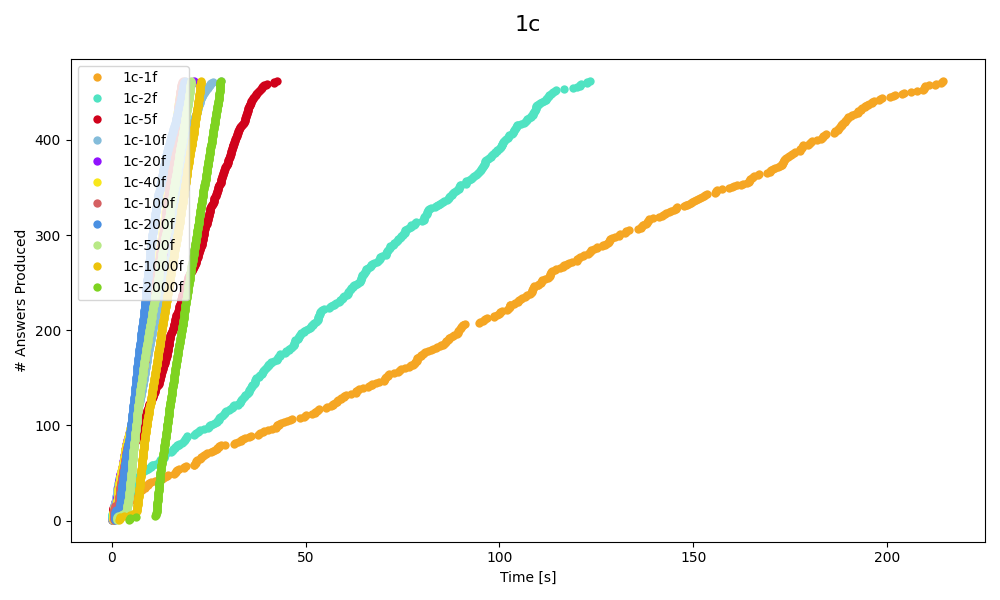
\includegraphics[scale = 0.5]{images/4-Experiments/E2/fixedcores/1c/traces.png}
  \caption{Alerts trace in time (s) - 1 core}
\end{figure}

\begin{figure}[H]
  \centering
  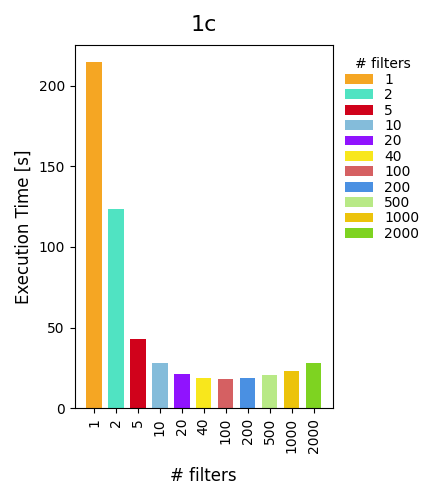
\includegraphics[scale = 0.5]{images/4-Experiments/E2/fixedcores/1c/execTime.png}
  \caption{Execution time (s) - 1 core}
\end{figure}

\begin{figure}[H]
  \centering
  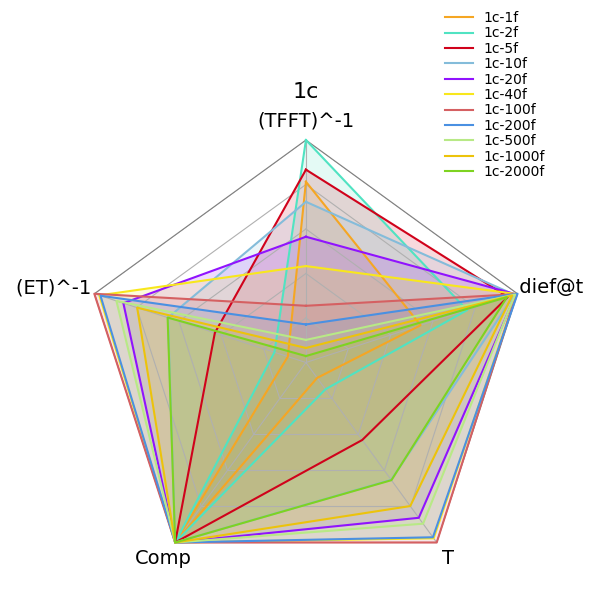
\includegraphics[scale = 0.5]{images/4-Experiments/E2/fixedcores/1c/radar-dieft.png}
  \caption{\texttt{dieft} radar - 1 core}
\end{figure}

\begin{figure}[H]
  \centering
  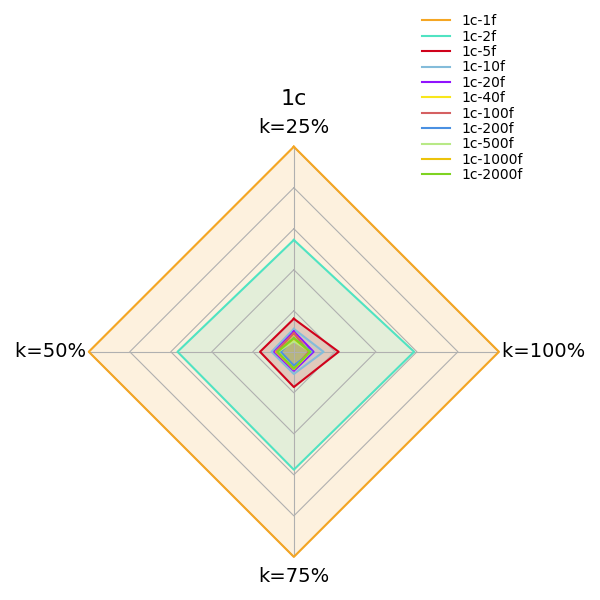
\includegraphics[scale = 0.5]{images/4-Experiments/E2/fixedcores/1c/radar-diefk.png}
  \caption{\texttt{diefk} radar - 1 core}
\end{figure}

\textcolor{red}{TODO: Put table for not graphical results gathered in the dieffpy-out.txt file...}

\paragraph{4-cores\\}

Results for executions with 4-core:

\begin{figure}[H]
  \centering
  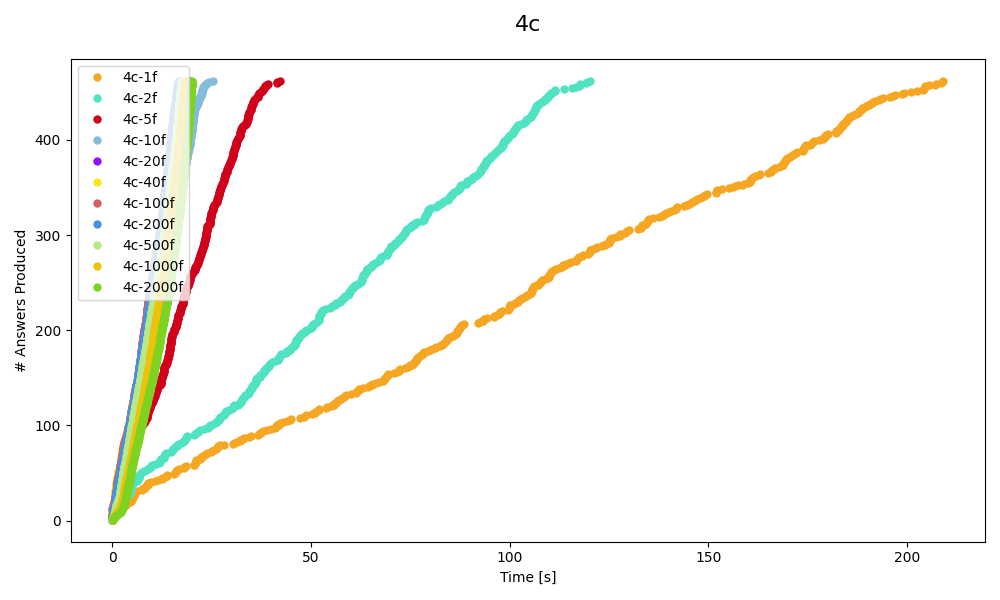
\includegraphics[scale = 0.5]{images/4-Experiments/E2/fixedcores/4c/traces.png}
  \caption{Alerts trace in time (s) - 4 core}
\end{figure}

\paragraph{8-cores\\}

Results for executions with 8-core:

\begin{figure}[H]
  \centering
  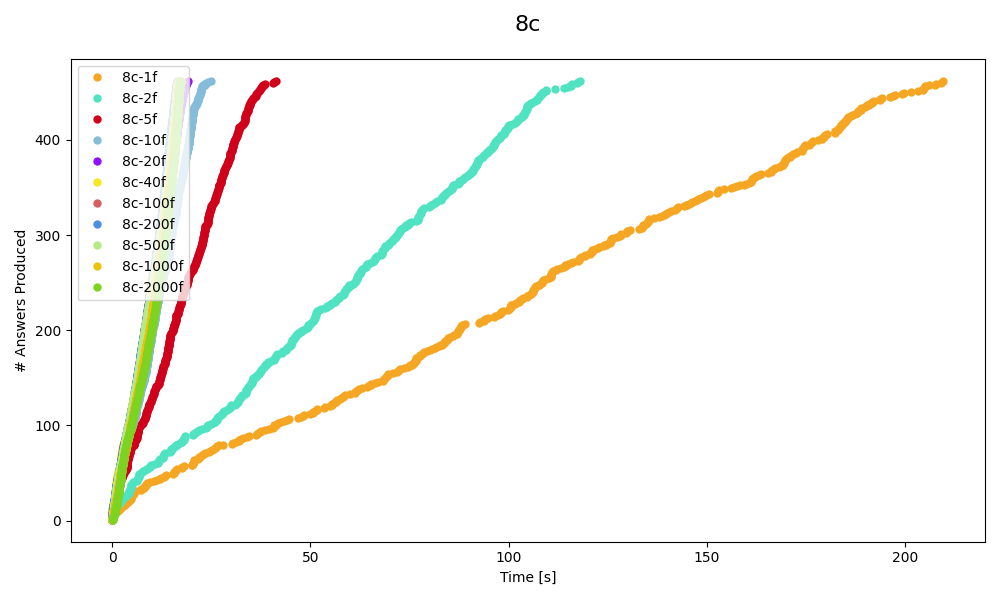
\includegraphics[scale = 0.5]{images/4-Experiments/E2/fixedcores/8c/traces.png}
  \caption{Alerts trace in time (s) - 8 core}
\end{figure}

\paragraph{16-cores\\}

Results for executions with 16-core:

\begin{figure}[H]
  \centering
  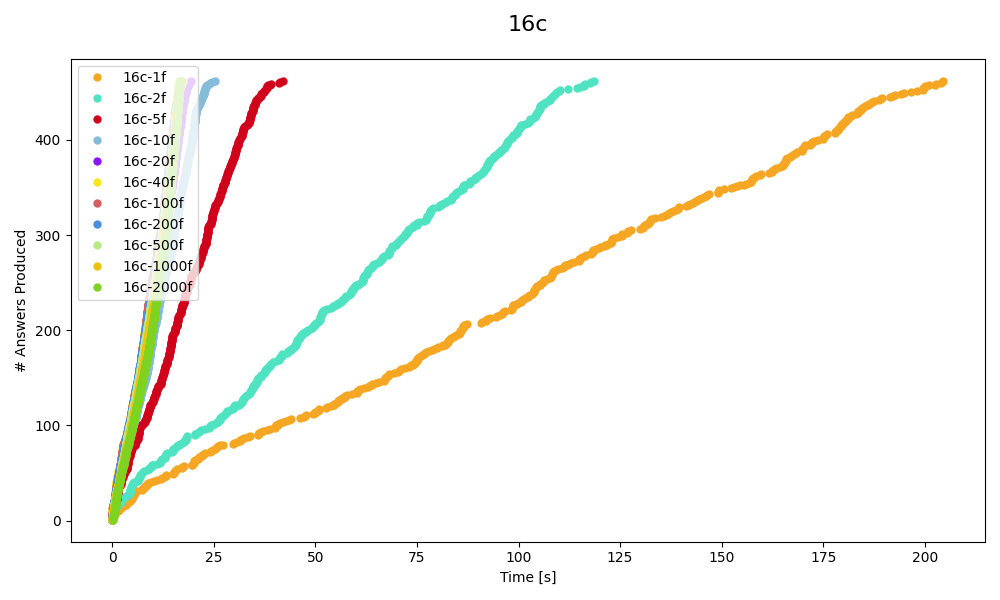
\includegraphics[scale = 0.5]{images/4-Experiments/E2/fixedcores/16c/traces.png}
  \caption{Alerts trace in time (s) - 16 core}
\end{figure}

\textcolor{red}{NOTE: Almost no difference when variating the number of cores!!!!}

\begin{figure}[H]
  \centering
  \begin{subfigure}[b]{0.45\textwidth}
    \centering
    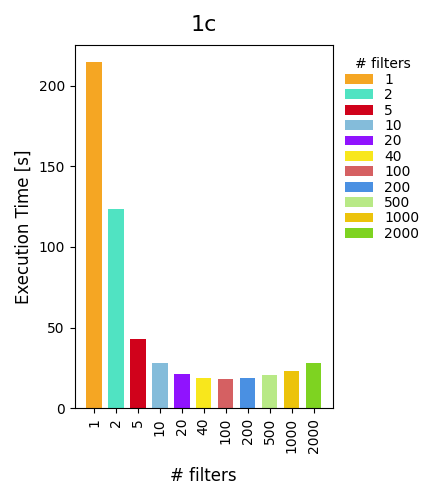
\includegraphics[scale=0.6]{images/4-Experiments/E2/fixedcores/1c/execTime.png}
    \caption{Execution time (s) - 1 core}
  \end{subfigure}
  \hfill
  \begin{subfigure}[b]{0.45\textwidth}
    \centering
    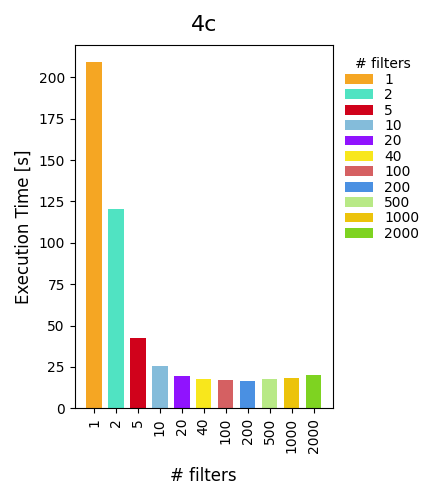
\includegraphics[scale=0.6]{images/4-Experiments/E2/fixedcores/4c/execTime.png}
    \caption{Execution time (s) - 4 core}
  \end{subfigure}
  \\
  \begin{subfigure}[b]{0.45\textwidth}
    \centering
    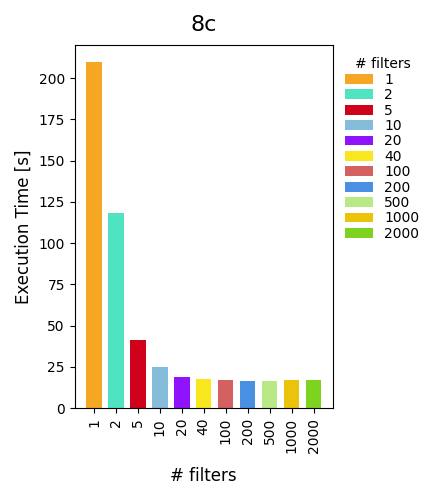
\includegraphics[scale=0.6]{images/4-Experiments/E2/fixedcores/8c/execTime.png}
    \caption{Execution time (s) - 8 core}
  \end{subfigure}
  \hfill
  \begin{subfigure}[b]{0.45\textwidth}
    \centering
    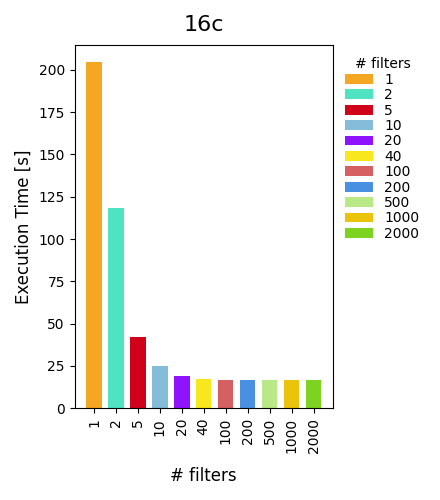
\includegraphics[scale=0.6]{images/4-Experiments/E2/fixedcores/16c/execTime.png}
    \caption{Execution time (s) - 16 core}
  \end{subfigure}
  \caption{Execution times for different core configurations.}
  \label{fig:execution-times}
\end{figure}


\textcolor{blue}{
Some observations:
\begin{itemize}
    \item Differences between  more or less cores visible specially for a fixed big number of filters (see plots of fixed number of filters) -> TODO
    \item More filters imply more overhead specially when number of cores is low.
\end{itemize}
}

\paragraph{Transaction stream - medium\\}

\begin{itemize}
  \item $\texttt{NUM\_DAYS} = 60$
  \item $\texttt{anomalous\_ratio} = 0.02\ (2\%)$ 
\end{itemize}

This setup gives us a transaction stream of 
\begin{itemize}
  \item $\texttt{total\_tx} = 80744$
  \item $\texttt{regular\_tx} = 79005$
  \item $\texttt{anomalous\_tx} = 1739$
\end{itemize}

\paragraph{Transaction stream - big\\}

\begin{itemize}
  \item $\texttt{NUM\_DAYS} = 120$
  \item $\texttt{anomalous\_ratio} = 0.02\ (2\%)$ 
\end{itemize}

This setup gives us a transaction stream of 
\begin{itemize}
  \item $\texttt{total\_tx} = 160750$
  \item $\texttt{regular\_tx} = 157756$
  \item $\texttt{anomalous\_tx} = 2994$
\end{itemize}

\textcolor{blue}{NOTE: only 5 runs each experiments instead of 10! - large execution time...}

\rule{\textwidth}{0.4pt} 
\textcolor{red}{$\rightarrow$ Issue: Connection timeout\\}
In the cases: 
\begin{itemize}
    \item 1c: $\ge 200f$
    \item 2c: $\ge 1000f$
\end{itemize}

Possible fixes:
\begin{itemize}
    \item (Optimization of the query... introducing indexing!)
    \item Increase the timeout
    \item Set a maximum connection pool size... Note that it may be needed for later experiments...
    Since we may not be able to open more than $x$ connections/sessions in parallel with the Neo4j gdb. Then we have 2 options:
    \begin{itemize}
        \item Limit the maximum number of filters based on this max limit on the number of parallel connections/sessions.
        \item Do not limit the maximum number of filters, but instead create a pool of connections.
    \end{itemize}
    \begin{enumerate}
        \item So far $\rightarrow$ Try to fix limiting the maximum timeout and limit the number of filters (with the idea that each filter has a permanent open session - instead of requesting a session from a pool of connections to a certain process manager of sessions every time it needs to query... - I think it is more clean and easy, and for the purposes of what we are doing to have a permanent open session per filter. So that:
        \begin{itemize}
            \item Easier to manage (apparently no limit on the number of parallel sessions - so no problem)
            \item We need to do a retry process - so that whenever the timeout exceeds it can try again without producing an error - and/or increase the timeout limit.
            \item Finally note that this problem is going to appear whenever we have many open threads connected in a high loaded scenario tested on a low-resource variant of the system (with few/low number of cores). And that, for a real scenario this is not going to be the case since the system will be expected to be way less loaded.
        \end{itemize}
    \end{enumerate}
\end{itemize}

\textcolor{green}{$\rightarrow$ Partial fix so far: increase the timeout of a transaction at the driver level to 1h: "config.MaxTransactionRetryTime = 1 * time.Hour"\\}

\textcolor{blue}{Some details about our Neo4j VM:
\begin{itemize}
    \item 4 cores and 20GB of RAM
    \item No limit on the number of parallel sessions. However it seems that by default there is a limit on the number of parallel transactions to 1000.
\end{itemize}
}

\subsection*{E2: Evaluation in a Real-World Stress Scenario}


E1: Mean Response Time

\begin{itemize}
  \item Q1: How much it takes for the system to emit the alerts from the moment the anomalous transaction was produced.
  \item R1: Real time simulation. Measuring the mean response time from the start of the transaction of the detected anomalous scenario until the alert is emitted by the system.
\end{itemize}


Note that, because of the way we did the transaction generator (coming from wisabi database client's behavior), the average number of transactions per day per card is $\sim1$, and therefore to be able to generate a transaction set with anomalous situations more close to reality, a reasonable time interval size for the generated transaction stream would be having $T$ around some weeks or month(s).

\subsubsection{E1: Mean Response Time}

\textbf{Real time-event stream simulation\\}
Since we do not have the material time to run each experiment for a interval time $T$ of some weeks or a month the idea is to do time scaling of the time event stream. We take the stream of a certain time interval size $T$ and map it into a smaller time interval
$T'$ where $T' << T$. Then, we do a real-time event simulation, providing the events of the input stream to the system at the times they actually occur (in reality possibly with a small certain delay!) using their timestamps.

\begin{itemize}
  \item \textbf{Shorter experimental time}: Reduced time to test the system behavior. Instead of $T$, only $T'$ time to test it. 
  \item \textbf{Stress testing - Graph database size - amount of filters' subgraphs}: We do not test the system under a real-case scenario considering its number of cards $c$, instead we are testing it under a higher load to what it would correspond, but having $c$ cards, and therefore $c$ filter's subgraph. The benefit is that we do not need to have such a big graph database.
\end{itemize}

The consequences for the experiments and metrics:

\begin{itemize}
  \item \textbf{Diefficiency metrics} (continuous delivery of results): If we give the input stream to the system respecting the temporal timestamps, note that no matter the system characteristics, that a result (an alert in our case), will not be possible to be produced until the event causing it arrives to the system. Therefore the emission of events is expected to be really similar in this case, for any system variation. Only in the case when the stream load is high enough we expect to see some differences?? \textcolor{orange}{$\rightarrow$ HABRÁ QUE IR VIÉNDOLO...}
  \item \textbf{Response time}: having in mind the previous considerations, we think in measuring the possible differences of behavior of the different system capabilities in terms of the mean response time. The mean response time (\texttt{mrt}) would be the average time that the system spends since it receives the transactions involved in an alert until the time it emits the alert.
\end{itemize}

\textcolor{red}{Problems derived to pay attention to}:
\begin{itemize}
  \item Shrinking the timestamps to a smaller time interval, produces the emergence of not real fraud patterns that before did not exist due to their real and "correct" larger time distance. Example:
  \begin{itemize}
  \item Consider the original size of the time interval of the input stream $T=120h$ (5 days) and $T'=24h$.
  \item Consider two consecutive regular transactions of a certain client performed in two different ATMs \texttt{ATM-x} and \texttt{ATM-y} with \texttt{t\_min}$=8$h (minimum time difference to traverse the distance from \texttt{ATM-x} to \texttt{ATM-y}) and \texttt{t\_diff}$=24$h (time difference between the first and the second transaction). 
  \item \textcolor{red}{$\rightarrow$ Note that with the scaling the time difference \texttt{t\_diff} would be of 5 times less, that is, $\texttt{t\_diff}=4.8h$. Therefore this will make $\texttt{t\_diff'}=4.8h < \texttt{t\_min}=8h$}.
  \end{itemize}
  \item $\rightarrow$ (*) Solution A: \textbf{introduce the scaling factor as a input parameter} and consider it also for the fraud checking so to properly \textbf{scale the $\texttt{t\_min}$ variable} ($\texttt{t\_min}=8h \rightarrow \texttt{t\_min'}=\frac{8}{5}h=1.6h$) and therefore: 
  \begin{itemize}
    \item Before scaling: $\texttt{t\_diff}=24h > \texttt{t\_min}=8h$.
    \item After scaling (scale factor $=\frac{1}{5}$): $\texttt{t\_diff}=24*\frac{1}{5}=4.8h > \texttt{t\_min}=8*\frac{1}{5}=1.6h$.
  \end{itemize}
  \item $\rightarrow$ Solution B: conserve the original timestamps, and consider the mapped-reduced timestamps for simulating the arrival times of the transactions into the system while taking the original timestamps for the checking of the frauds.
\end{itemize}

\begin{tcolorbox}[colframe=red!75]
\textcolor{red}{\textbf{IMPORTANT: WHAT DO WE WANT TO TEST?\\}}
Definition of the objectives of the experiments:
\begin{itemize}
    \item See and compare the behavior of the system(s) with different streams (different number of cards, greater or smaller size of the bank - and therefore its database). \\
    \begin{itemize}
        \item Alert/result response time comparison. \textbf{Continuous delivery of results (diefficiency metrics) does not make sense!}. With the objective to see that we can see lower response time in the case of the dp versions.
    \end{itemize}
\end{itemize}
\end{tcolorbox}

\ad{Esto tiene que ir al principio de la sección de experimentos, tienes que explicar "con palabras" qué es lo que quieres probra y luego cómo lo haces.}

\paragraph{Problems derived:\\}
\begin{itemize}
    \item \textbf{Continuous delivery of results comparison does not make sense.} $\rightarrow$ In a real time simulation, for any system, results can only be emitted whenever the corresponding anomalous transaction $a_i$ reaches the system. That happens at the same time $t_i$ for both approaches when the input stream is simulated at real time, meaning that the result corresponding to the anomalous transaction $a_i$ can not be emitted in any case before time $t_i$. Therefore, the difference in time delivery of this result between the different approaches is not expected to be high unless we make the systems to be loaded enough. \textbf{Therefore, for small sized banks this does not really make sense...}
    \item \textbf{Losing of alerts}: Due to scaling we are losing alerts since we have seconds precision. We will have to scale to the millisecond or nanosecond the timestamps to possibly do not loose those alerts, due to time scaling precision.
    \item \textbf{Although scaling, the load we are simulating is higher than real... - like for the not real time approach}
\end{itemize}

\subsubsection{Initial experiments}

\textit{Small} initial graph database (gdb) size:
\begin{itemize}
  \item $|ATM| = 50$
  \item $|Card| = 2000$
\end{itemize}

Transaction stream:
\begin{itemize}
  \item $\texttt{NUM\_DAYS} = 30$
  \item $\texttt{anomalous\_ratio} = 0.02\ (2\%)$ 
\end{itemize}

This setup gives us a transaction stream of 
\begin{itemize}
  \item $\texttt{total\_tx} = 39959$
  \item $\texttt{regular\_tx} = 39508$
  \item $\texttt{anomalous\_tx} = 451$ -- note that this is actually a $1\%$.
\end{itemize}

\begin{table}[H]
\centering
\begin{tabular}{|c|c|c|c|c|c|}
  \hline
  Execution & Scaled   & Num. cards/filter& Num. cores & Num. alerts & Time(s) \\ \hline
  NRT & No & Baseline (all) & 1 & 462 & 44.88 \\ \hline
  RT  & 1h & Baseline (all) & 1 & 447 & 3601.65\\ \hline
  RT  & 1h & 500 (4 filters) & 4 & 447 & 3603.25\\ \hline
  RT  & 1h & 200 (10 filters) & 10 & 447 & 3602.71\\ \hline
  RT  & 6h & Baseline (all) & 1 & 459 & 21606.11 \\ \hline
  RT  & 6h & 500 (4 filters) & 4 & 459 & 21611.75 \\ \hline
  RT  & 12h & Baseline (all) & 1 & 461 & 43211.95 \\ \hline
\end{tabular}
\caption{Different experimental setups results}
\label{table:small-results}
\end{table}

Some nomenclature:
\begin{itemize}
  \item NRT: Not Real Time execution
  \item RT: Real Time execution
\end{itemize}

Some results:

\paragraph{1h scaling\\}

\ad{Los captions de las figuras tienen que ser autocontenidos.}


\begin{figure}[H]
  \centering
  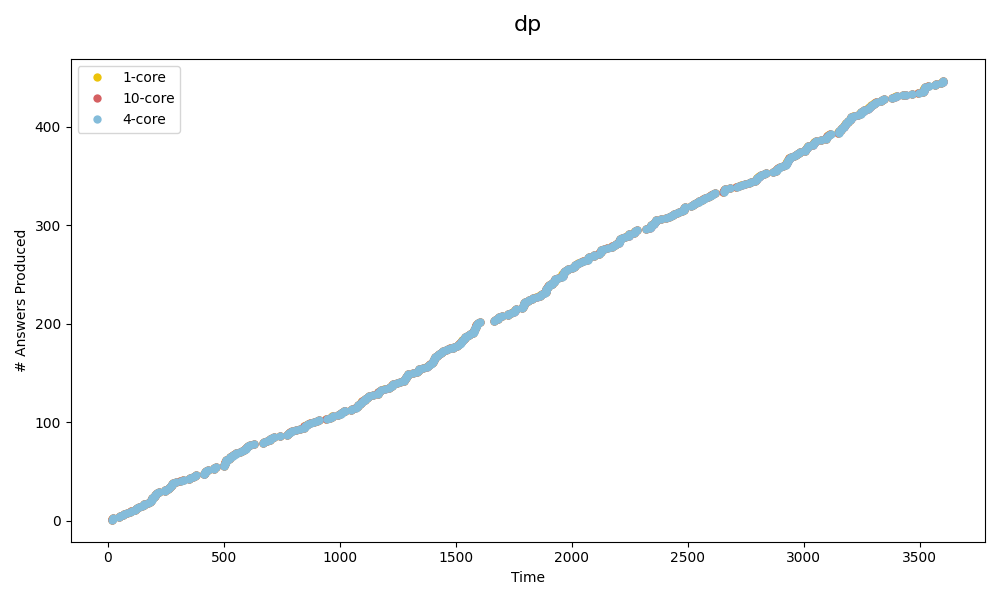
\includegraphics[scale = 0.5]{images/4-Experiments/traces-1h.png}
  \caption{Trace 1h}
\end{figure}

Only for the first 10 results (alerts):
\begin{figure}[H]
  \centering
  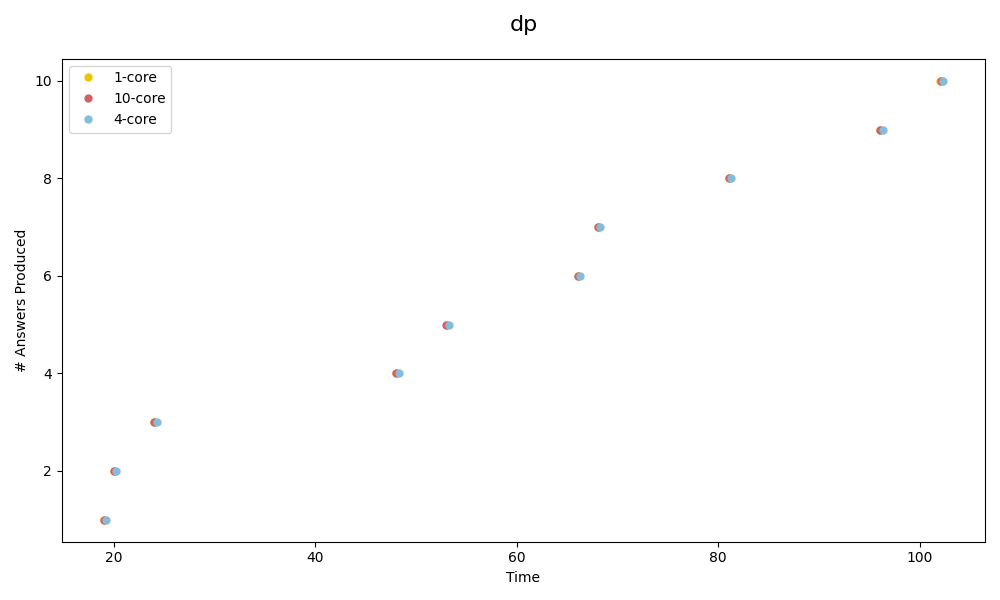
\includegraphics[scale = 0.5]{images/4-Experiments/traces-1h-10.png}
  \caption{Trace 1h - first 10 alerts}
\end{figure}

\paragraph{6h scaling\\}

We do not see any difference in the behavior between the baseline with 1 filter and 1 core approach (\texttt{RT-6h-1c-1f}) and the approach with 4 filters and 4 cores (\texttt{RT-6h-4c-4f}). 

\textbf{WHY?} $\rightarrow$ a possible reason is that results can only be emitted whenever the corresponding anomalous transaction $a_i$ reaches the system. That happens at the same time $t_i$ for both approaches when the input stream is simulated at real time, meaning that the result corresponding to the anomalous transaction $a_i$ can not be emitted in any case before time $t_i$. Therefore, the difference in time delivery of this result between the different approaches is not expected to be high unless we make the systems to be loaded enough.

\subsection{Definitive Experiments}

$\rightarrow$ We set the worker stream reading by chunks, with chunk size of $10^2$.\\

The setups of the experiments that we are going to do are:
\begin{itemize}
  \item Fix different bank sizes (small, $+\frac{1}{4}$, $+\frac{2}{4}$, $+\frac{3}{4}$, the biggest possible size).
  \begin{itemize}
    \item For each, generate different stream sizes.
    \begin{itemize}
      \item Compare different system variations in the number of cores and number of filters.
    \end{itemize}
  \end{itemize}
\end{itemize}

\begin{table}[H]
\centering
\begin{tabular}{|c|c|c|c|}
\hline
Bank Size & \# Cards & \# ATMs & Stream Size (\# tx) \\ \hline
Small     & 2000     & 50 (45 internal - 5 interbank)     & 39959 - small       \\ \hline
Small     & 2000     & 50 (45 internal - 5 interbank)      & 80744 - medium      \\ \hline
Small     & 2000     & 50 (45 internal - 5 interbank)     & 160750 - big        \\ \hline
Medium    & 500000   & 1000 (900 internal - 100 interbank)   &                     \\ \hline
          &          &         &                     \\ \hline
          &          &         &                     \\ \hline
Big       &          &         &                     \\ \hline
Big       &          &         &                     \\ \hline
Big       &          &         &                     \\ \hline
\end{tabular}
\end{table}

\subsubsection{Bank size: Initial - Small}

\begin{itemize}
  \item $|ATM| = 50$
  \item $|Card| = 2000$
\end{itemize}

\paragraph{Transaction stream - small\\}

\begin{itemize}
  \item $\texttt{NUM\_DAYS} = 30$
  \item $\texttt{anomalous\_ratio} = 0.02\ (2\%)$ 
\end{itemize}

This setup gives us a transaction stream of 
\begin{itemize}
  \item $\texttt{total\_tx} = 39959$
  \item $\texttt{regular\_tx} = 39508$
  \item $\texttt{anomalous\_tx} = 451$ -- note that this is actually a $1\%$.
\end{itemize}

For different core variations, we are going to try different combinations of the system in terms
of the number of the maximum number of cards per filter, that consequently will produce an inverse variation in the number of filters of the system.

\begin{table}[H]
  \renewcommand{\arraystretch}{1.5} % control row height
  \centering
  \begin{tabular}{|c|c|}
  \hline
  \# cards per filter & \# filters \\ \hline
  2000   &   1     \\ \hline
  1000   &   2     \\ \hline
  400 &   5     \\ \hline
  200  &   10     \\ \hline
  100 &   20    \\ \hline
  50  &   40    \\ \hline
  20  &   100    \\ \hline
  10  &   200    \\ \hline
  4  &   500    \\ \hline
  2  &   1000    \\ \hline
  1  &   2000    \\ \hline
  \end{tabular}
\end{table}

\begin{itemize}
  \item \# of times / runs each job $=10$.
  \item Maximum RAM limited to 16GB.
\end{itemize}

\subsection{E1: Mean Response Time}

\begin{itemize}
  \item Q1: How much it takes for the system to emit the alerts from the moment the anomalous transaction was produced.
  \item R1: Real time simulation. Measuring the mean response time from the start of the transaction of the detected anomalous scenario until the alert is emitted by the system.
\end{itemize}

Setting up the experiments:

\begin{itemize}
    \item Scaling issue: \textcolor{green}{- Fixed - scaled at the level of the $\mu$s}
\end{itemize}

\subsubsection{Small bank size \& small transaction stream}

\begin{itemize}
    \item Scaling to 600s (10 minutes) $\rightarrow$ no losing of alerts (462).
\end{itemize}

\textcolor{blue}{
My doubts on these experiments
\begin{itemize}
    \item Results = Checks: same issue as with the alerts, a same check(tx1,tx2) on a card can not be performed until the tx2 reaches the system, which is the same simulated time on any system.
    \item For a small bank size, as the simulation tends to be closer to reality (lower scaling), 
    then the system has lower overhead and the differences between the different variations will be almost negligible. Also the time needed to perform these simulations increases.
    \item However, on the contrary, when the scaling is high, then the simulation is farther from reality, making the system to be more loaded than in a real case scenario, reaching a point that the experiment will be almost the same as E2 (reading the transaction stream input directly without any real-time simulation).
    \item To have a "real-time" simulation in which differences between the systems can be observed we will need to simulate a big bank, which is able to provide a dense/big stream, which intuitively, even more if the stream is scaled, the simulation will be almost like reading the stream directly from the input like without any "real-time" simulation, like in the case of the E2 experiments. 
\end{itemize}
}

\textcolor{orange}{
Proposals:
\begin{itemize}
    \item Do more variations on the stream size and bank database size for the E2 experiments.
    \begin{itemize}
        \item Incrementing the database size, is expected to increase the overhead due to the greater number of cards and the latency to query the stable bank database.
        \item Increasing the stream size...?
    \end{itemize}
    \item On the E2 experiments measure and compare the response time for providing an alert (the time since the last transaction producing the alert happened until the time the system emits out that alert). \textbf{But focusing only on the alerts and not on all the checks, I think it is sufficient to compare only on the alerts.} Also measuring on the checks will introduce an overhead on the needed message passing from the filters to the sink to do all this gathering on these times, whereas with the alerts it is minimal since they are already sent to the Sink stage.
\end{itemize}
}

Some experiments that were tested:

\begin{itemize}
    \item Scaled small bank data stream of 30 days to 10 minutes.
    \item Tested for these combinations:
    \begin{table}[H]
      \renewcommand{\arraystretch}{1.5} % control row height
      \centering
      \begin{tabular}{|c|c|}
      \hline
      \# cores & \# filters \\ \hline
      1        & 1  \\ \hline
      4        & 40  \\ \hline
      16       & 2000  \\ \hline
      \end{tabular}
    \end{table}
\end{itemize}

\rule{\textwidth}{0.4pt} 

\subsection{Update: Recording all the checks}

\subsection{How to measure MRT}\label{exp-measuring-mrt}

To show the continuous delivery of results of the system, for testing purposes, instead of only recording the alerts (positive fraud checks) in the Sink, we are now going to be recording all the check results whether they are positive (alerts) or negative.\\
How we do this?\\
Measurement options:
\begin{itemize}
    \item Measure the \texttt{time.End} of the check on the Sink. As with the alerts is the time it takes for the system to emit the result.
    \item Measure the \texttt{time.End} of the check on the Filter. It could be argued that the alerts (which are the unique results that in reality get out of the system) could be directly be sent from the Filters and not from the Sink, saving the time they need to travel to the Sink inside the system. Anyway they will need to travel to the Sink to be registered on the bank system but the alert to the user could be directly sent faster from the Filters.
\end{itemize}

So far:
\begin{itemize}
    \item Measurement: done at the Sink.
    \item Register of the results at the Sink and sent all (positive and negative) through a unique channel from each Filter to the Sink (we reuse the \texttt{alert} channel).
\end{itemize}

Some experiments were done to inspect whether there was a significant difference on the measurement position. In particular, we measured the response time of each of the checks both in the Filter and in the Sink, to finally obtain the mean response metrics times of both approaches. In the table \ref{tab:response-time-measurement-comparison} we show the mean response time metric in ms measured at the Sink (\texttt{mrt-Sink}) and the difference of this measurement on average with respect to the measurement done in the Filter in ms (\texttt{mrt-difference}).

Note that each of this experiments were done running in not-real-time, with the small bank size, and the \texttt{30-0.02} stream. Each of the experiments were run 10 times... 16GB RAM...

\textcolor{blue}{As it can be observe the differences are negligible, and therefore for simplicity, and to maintain the "philosophy" of the dynamic pipeline, we decided to keep the measurement of the response times of the checks on the Sink stage.}

\textcolor{red}{Note that, measuring in the Filter would imply assuming that the alerts had to be sent from there, to be realistic to where we are measuring.}
\textcolor{red}{Note that: measuring all the results and not only the alerts imply unnecesarily overloading the system, since only sending the alerts to the Sink should be enough for the purposes of our application. However, due to experimental purposes we are forced to send/measure all the checks, in order to be able to compare the continuous delivery of results of all the system configurations/variations}.

\begin{table}[H]
\centering
\begin{tabular}{|c|c|c|c|}
\hline
\# filters & \# cores & \begin{tabular}[c]{@{}c@{}}mrt-Sink\end{tabular} & \begin{tabular}[c]{@{}c@{}}mrt-difference\end{tabular} \\ \hline
1          & 1        & 24899.103                                                         & 0.071                                                                          \\ \hline
1          & 4        & 24077.638                                                         & 0.041                                                                          \\ \hline
1          & 16       & 22302.060                                                         & 0.016                                                                          \\ \hline
40         & 1        & 8852.990                                                          & 0.195                                                                          \\ \hline
40         & 4        & 8012.537                                                          & 0.065                                                                          \\ \hline
40         & 16       & 8241.212                                                          & 0.040                                                                          \\ \hline
2000       & 1        & 13949.781                                                         & 2.229                                                                          \\ \hline
2000       & 4        & 10464.550                                                         & 0.847                                                                          \\ \hline
2000       & 16       & 7982.963                                                          & 0.052                                                                          \\ \hline
\end{tabular}
\caption{Comparison of the response time measurement positions with different system configurations}
\label{tab:response-time-measurement-comparison}
\end{table}

\subsubsection{Bank size: Medium}

\textcolor{red}{For these experiments, to generate the stream of tx, we needed to simplify this process in order to be able to generate a stream in a feasible amount of time. In particular we used the simplifed version of the \texttt{txGenerator.py}: \texttt{txGenerator-simplified.py} $\rightarrow$ with a random ATM-subset instead of a closest to client ATM-subset. Also variation on the transaction distribution times.}


\begin{itemize}
  \item $|ATM| = 1000$
  \item $|Card| = 500000$
\end{itemize}

\begin{table}[H]
  \renewcommand{\arraystretch}{1.5} % control row height
  \centering
  \begin{tabular}{|c|c|}
  \hline
  \# cards per filter & \# filters \\ \hline
  500000   &   1     \\ \hline
  100000   &   5     \\ \hline
  50000 &   10     \\ \hline
  5000  &   100     \\ \hline
  2000 &   250    \\ \hline
  1000  &   500    \\ \hline
  500  &   1000    \\ \hline
  250  &   2000    \\ \hline
  100  &   5000    \\ \hline
  50  &   10000    \\ \hline
  10  &   50000    \\ \hline
  \end{tabular}
\end{table}

\paragraph{Transaction stream - small\\}


\begin{itemize}
  \item $\texttt{NUM\_DAYS} = 15$
  \item $\texttt{anomalous\_ratio} = 0.03\ (3\%)$ 
\end{itemize}

This setup gives us a transaction stream of 
\begin{itemize}
  \item $\texttt{total\_tx} = 4856573$
  \item $\texttt{regular\_tx} = 4805920$
  \item $\texttt{anomalous\_tx} = 50653$
\end{itemize}

First run:
\begin{itemize}
    \item 16GB RAM
    \item 16 cores
    \item Experiments for $|filters|\ge100$
    \item x1 run each job
\end{itemize}

\begin{table}[H]
\begin{tabular}{|c|c|c|c|c|c|c|c|c|c|c|c|}
\hline
\#cores & 1f & 5f & 10f & 100f & 250f & 500f & 1000f & 2000f & 5000f & 10000f & 50000f \\ \hline
1       &    &    &     &      &      &      &       &       &       &        &        \\ \hline
2       &    &    &     &      &      &      &       &       &       &        &        \\ \hline
4       &    &    &     &      &      &      &       &       &       &        &        \\ \hline
8       &    &    &     &      &      &      &       &       &       &        &        \\ \hline
16      & R & R & R & OK & OK & OK & OK & OK & OK & OK & outMem \\ \hline
\end{tabular}
\end{table}

\textcolor{red}{TO TRY:}
\begin{itemize}
    \item 32 or 64 RAM
    \item 16 cores
    \item Experiments for $|filters|\ge100$
\end{itemize}


\subsection{How to run the experiments}

\begin{itemize}
    \item Run \texttt{\$> launchAll-\{1,2,4,...\}c.sh <descriptions> <execTimes>} where we select the script to run based on the number of cores (1,2,4...) and maximum RAM with which to run the set of experiments. Indicate the directory of the description files of the experiments to run with \texttt{<descriptions>}, and the number of times to run each experiment with the \texttt{<execTimes>} parameter.
    Each description file of an experiment has to be in a csv format indicating \texttt{txFile,test,approach,maxFilterSize} where:
    \begin{itemize}
        \item \texttt{txFile}: indicates the name of the input stream file.
        \item \texttt{test}: label indicating the name of the test we perform (stream input and cores)
        \item \texttt{approach}: label indicating the name of the approach we perform (cores and filters)
        \item \texttt{maxFilterSize}: to set the maximum number of cards per filter. To set up the maximum number of filters for the tested system.
    \end{itemize}
    An example of a csv experiment description file is shown in \ref{csv-exp-description}.
    \begin{center}
    \lstset{style=cypherStyle}
    \begin{lstlisting}[caption={30-0.02-1c-4f}, label={csv-exp-description}]
        txFile,test,approach,maxFilterSize
        ../input/small/30-0.02.csv,30-0.02-1c,1c-4f,500
    \end{lstlisting}
    \end{center}
    \item Run \texttt{\$> summary-results.sh <directory> <TEST>}: to obtain the averaged results of the experiments run stored in the indicated output \texttt{<directory>} (the predefined output directory is the called \texttt{output} directory) and then \texttt{<TEST>} where we need to indicate the name of the performed test (like in the experiments description files).
\end{itemize}



\subsection{Input reading by chunks}\label{exps-input-reading}

In a real-case scenario, these interaction events could be sent by the ATMs of the bank network and be received by a message queue on our \DPATM system. For our proof of concept, where we generated our own synthetic stream of transactions in a \texttt{csv} file,
the interactions are read from these files, parsed into \texttt{Edge} data types and provided to the pipeline in different ways depending on the kind of simulation we perform. As it will be shown in the Experiments section, we implemented two different cases of simulations. The real-case scenario and the high loaded test scenario. In the first case, the interactions, although read by a file of artificial simulated interactions, are provided to the pipeline data stream in such a way that they simulate their actual arrival time to the system, with the corresponding time separation between them. In the second case, the interactions are provided just one after the other as fast as possible as they are read.\\

% Cómo se leen, parsing al tipo de dato Edge...
In any case, we want the reading of the input file to be the fastest possible, so to minimize the potential bottleneck derived from the operation of reading a file, we utilized a buffered reader of the \texttt{bufio} package, which reads chunks of data into memory, providing buffered access to the file. This buffered reader was provided to a \texttt{csv} reader of the \texttt{encoding/csv} package to read the buffered stream as \texttt{csv} records.

    \begin{center}
    \lstset{style=golangStyle}
    \begin{lstlisting}[caption={\texttt{csv-bufio} reader}]
        reader := csv.NewReader(bufio.NewReader(file))
    \end{lstlisting}
    \end{center}
    
% Lectura por chunks
% chunk size = 100
% read with the help of a worker to keep reading in the background, to accelerate the reading -> explain the reason of why this
Another optimization that was done in order to be able to minimize this bottleneck on the reading of the interactions from the \texttt{csv} file, was reading by chunks the \texttt{csv} records/rows. In particular, this was done by having a \textit{worker} subprocess, implemented as an anonymous \texttt{goroutine} inside \Sr, whose task was to continuously read records from the file using the \texttt{csv-bufio} reader accumulating them in a chunk of rows that were provided through a channel to \Sr whenever they reached the defined \emph{chunkSize}. These records were read directly as \texttt{string} data types. On its side, whenever \Sr receives a chunk of rows, it takes each of the rows on it, parses it to the \texttt{Edge} data type and sends it through the pipeline to the next stage.\\

The \emph{chunkSize} was selected to be of $10^2$ rows. In \ref{exps-input-reading} we provide an experimental analysis that proves and justifies the benefits of this buffered and chunked file reading. On it the \texttt{encoding/csv} package performance is compared to other variants using the \texttt{apache/arrow} package with different combinations of \emph{chunkSize}. We also analyze the benefits of introducing the \textit{worker} subprocess to perform the chunked reading.

\begin{itemize}
  \item \href{https://medium.com/@anuragv.1020/chunk-by-chunk-tackling-big-data-with-efficient-file-reading-in-chunks-c6f7cf153ccd}{Chunk-by-Chunk: Tackling Big Data with Efficient File Reading in Chunks}
  \item \href{https://pkg.go.dev/github.com/apache/arrow/go/arrow/csv#NewReader}{csv chunk reader - with Apache Arrow package}
\end{itemize}

\subsubsection{Apache Arrow}

\href{https://pkg.go.dev/github.com/apache/arrow/go/v12@v12.0.1/arrow/csv}{Apache arrow CSV}
package allows reading csv in chunks of $n$ rows, called \emph{records}.

The thing is that \emph{records} / apache arrow is optimized storing the data in a columnar way (by columns). So that we can not access the original $n$ rows easily, but instead the columns of these rows. And therefore, from them we will need to reconstruct the rows by taking the corresponding elements from each of the columns, given the index of the corresponding row.

Good references:
\begin{itemize}
  \item \href{https://www.apachecon.com/acna2022/slides/01_Topol_Arrow_and_Go.pdf}{Apache Arrow and Go - Good tutorial}
\end{itemize}


\subsubsection{encoding/csv}

\subsubsection{Experiments over the different approaches}

Approaches:
\begin{itemize}
  \item \texttt{1-apache/arrow} direct reading of corresponding data type in the worker.
  \item \texttt{2apache/arrow} reading as string data type. Later conversion in main.
  \item \texttt{3-encoding/csv}: row by row reading and passing chunks of rows to main.
\end{itemize}

\textcolor{red}{TODO: put a schema of the main/worker to show the different approaches better}

\begin{itemize}
  \item For the different approaches we tried with different sizes of files: $10^4$, $10^5$ and $10^6$ number of rows (transactions).
  \item For each of the sizes we compared the time it took to read the full file to each of the variants, testing for different chunk sizes in terms of the number of rows: ranging from $10^0, 10^1, 10^2,...$ up to the total number of rows of the file (maximum possible chunk size, all at once).
  \item Each of the experiments is done 20 times to obtain stable measurements.
\end{itemize}


\begin{figure}[H]
  \centering
  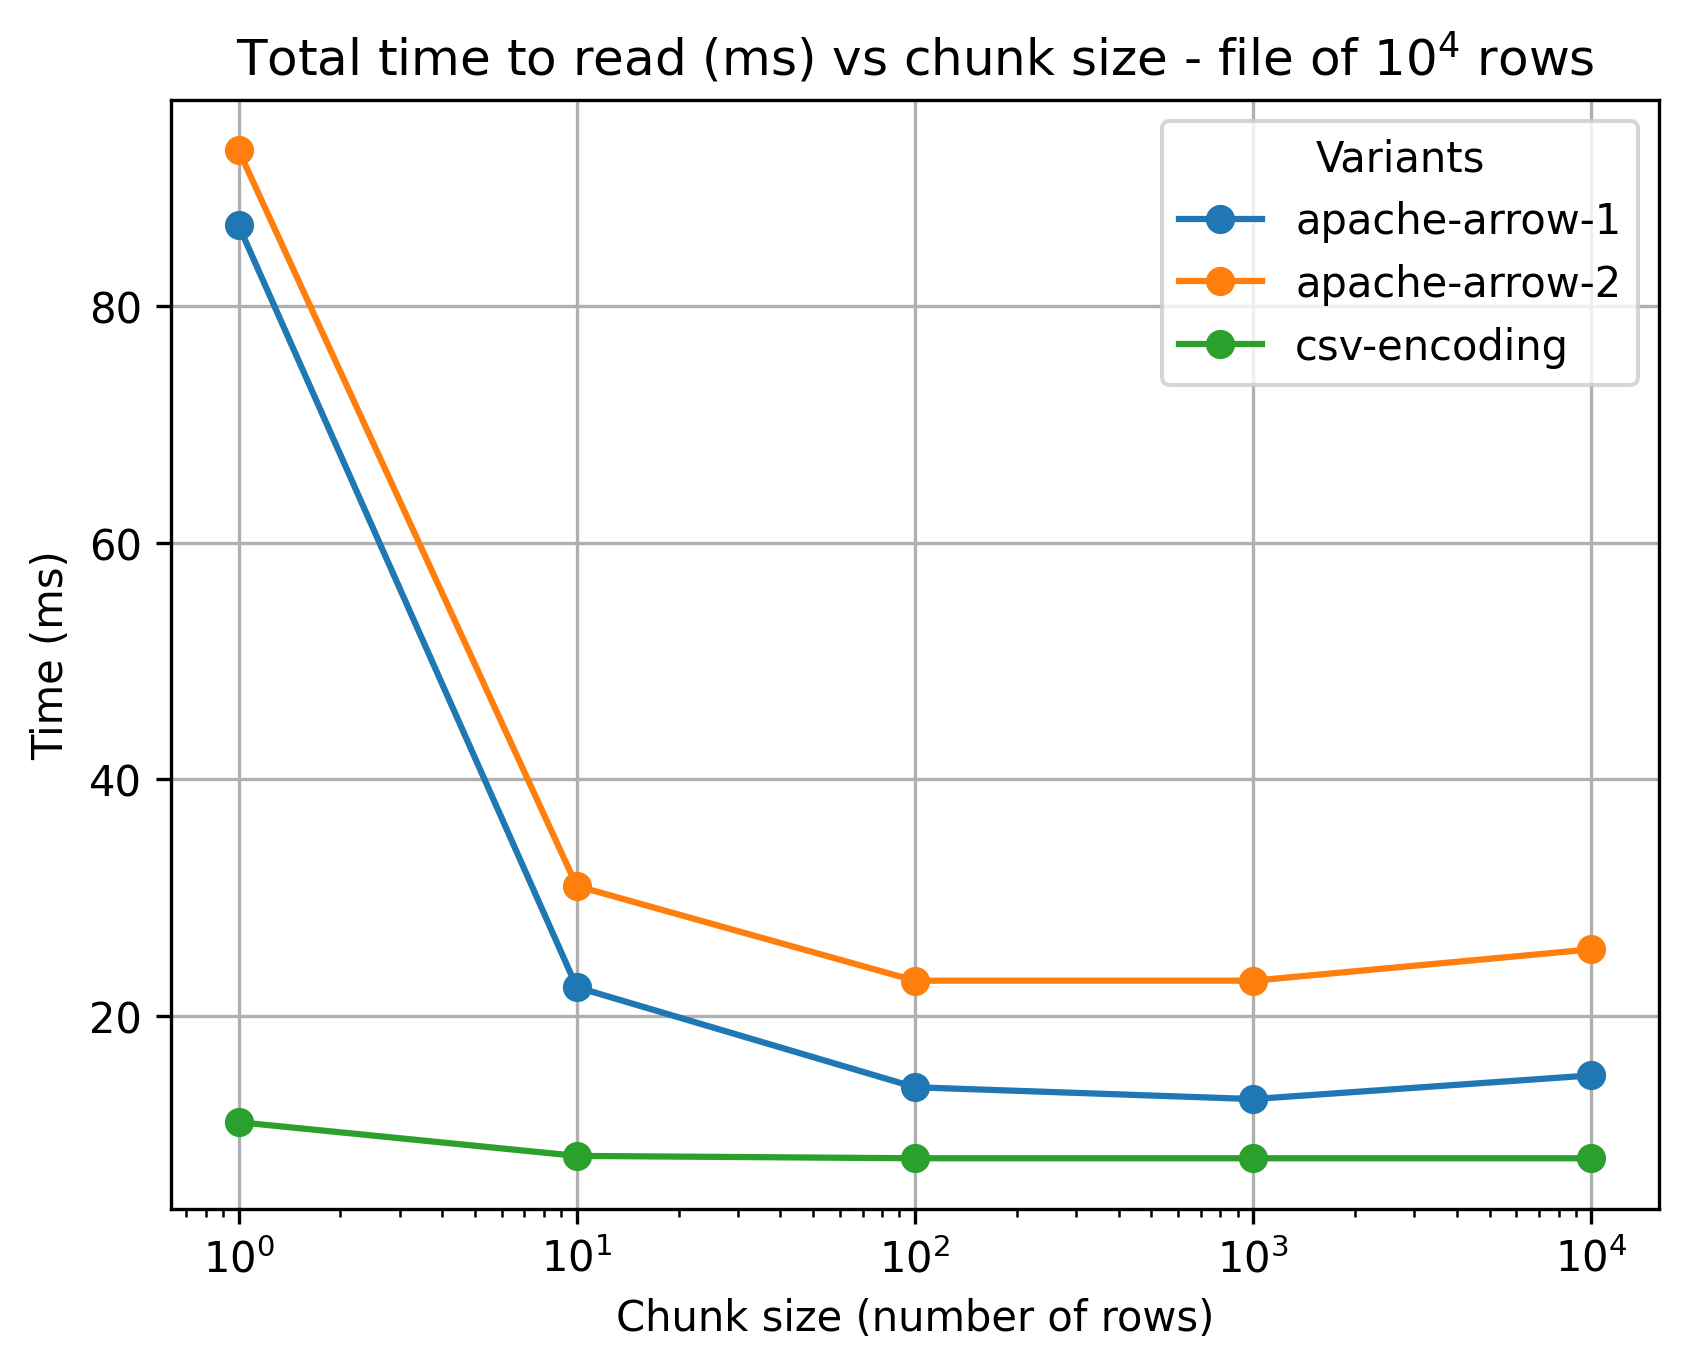
\includegraphics[scale = 0.7]{images/4-Experiments/read-input-10-4.png}
  \caption{Comparison of the variants for file of $10^4$ rows}
\end{figure}

\begin{figure}[H]
  \centering
  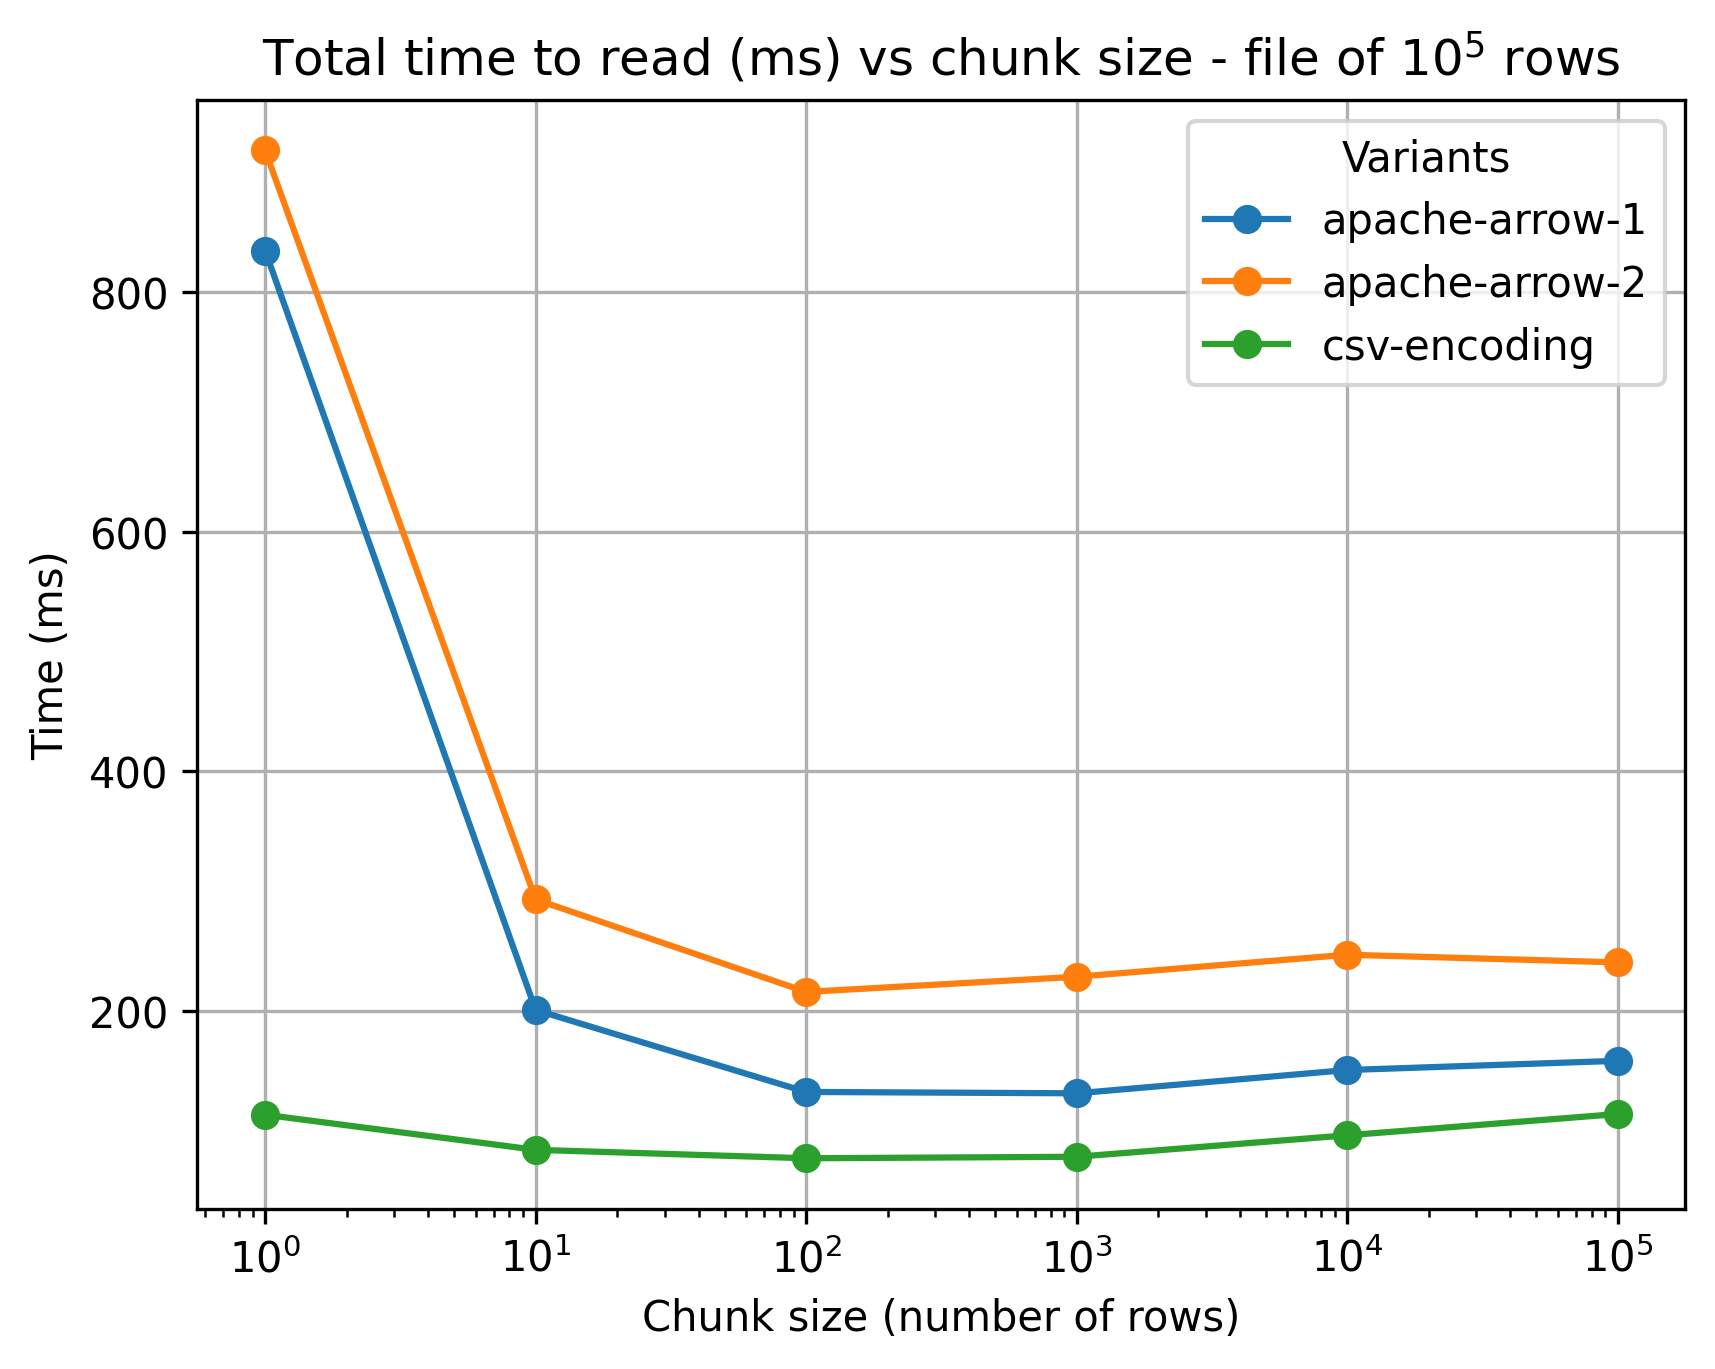
\includegraphics[scale = 0.7]{images/4-Experiments/read-input-10-5.png}
  \caption{Comparison of the variants for file of $10^5$ rows}
\end{figure}

\begin{figure}[H]
  \centering
  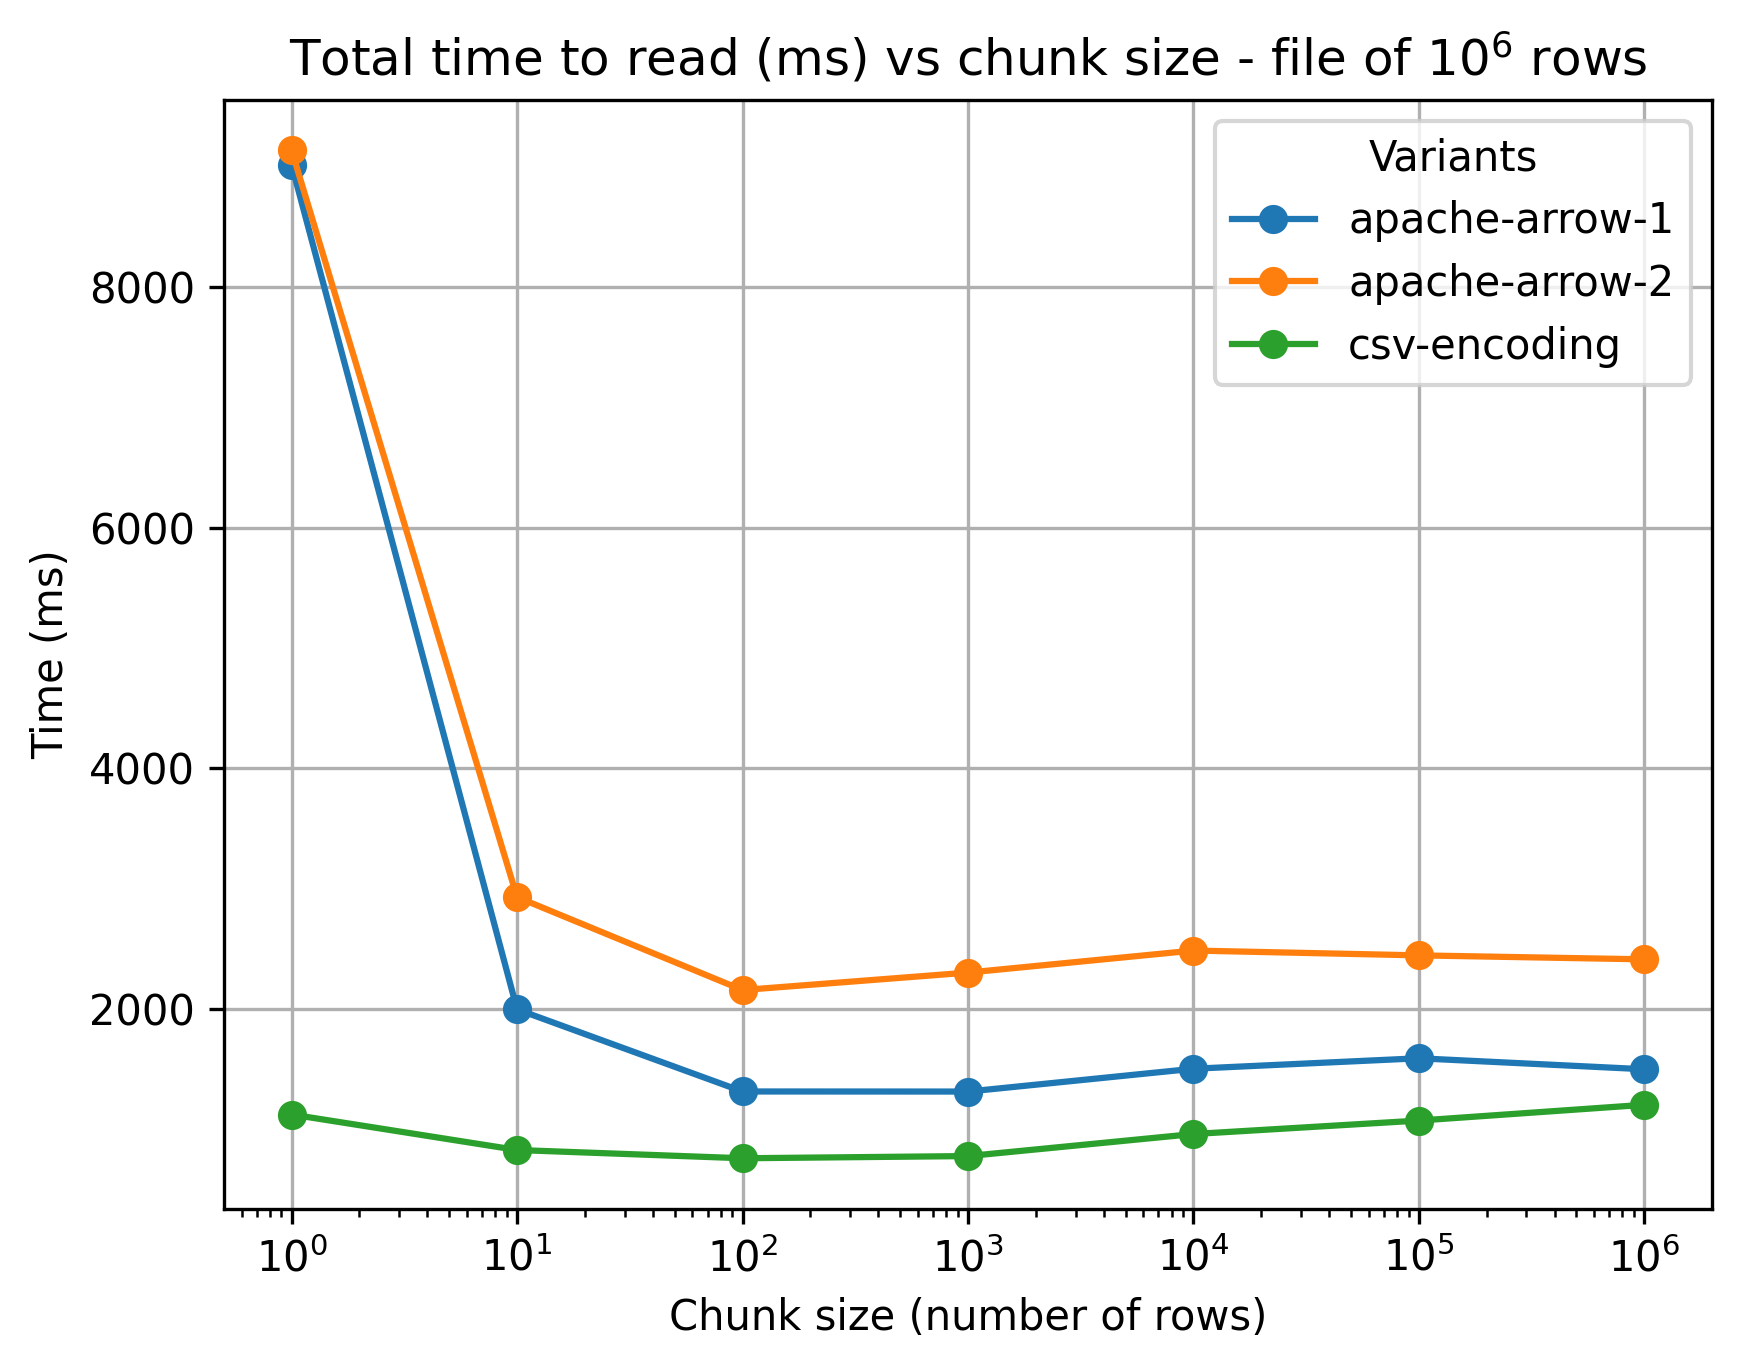
\includegraphics[scale = 0.7]{images/4-Experiments/read-input-10-6.png}
  \caption{Comparison of the variants for file of $10^6$ rows}
\end{figure}

Note that in all of the cases, the fastest approach is the one using the \texttt{csv/encoding} library. And, in addition, with chunk size of $10^2$ rows.

Once we decided to use the approach using the \texttt{csv/encoding} library, we performed an additional experiment in order to see if it was actually worthy to do the \emph{background} reading of the input with a worker goroutine. To see this:

\begin{itemize}
  \item Compare the variant with worker and chunk size of $10^2$ with the one without worker and therefore not reading by chunks.
  \item Comparison for different sizes of files: $10^4$, $10^5$ and $10^6$ number of rows (transactions).
  \item Each of the experiments is done 20 times to obtain stable measurements.
\end{itemize}

\begin{figure}[H]
  \centering
  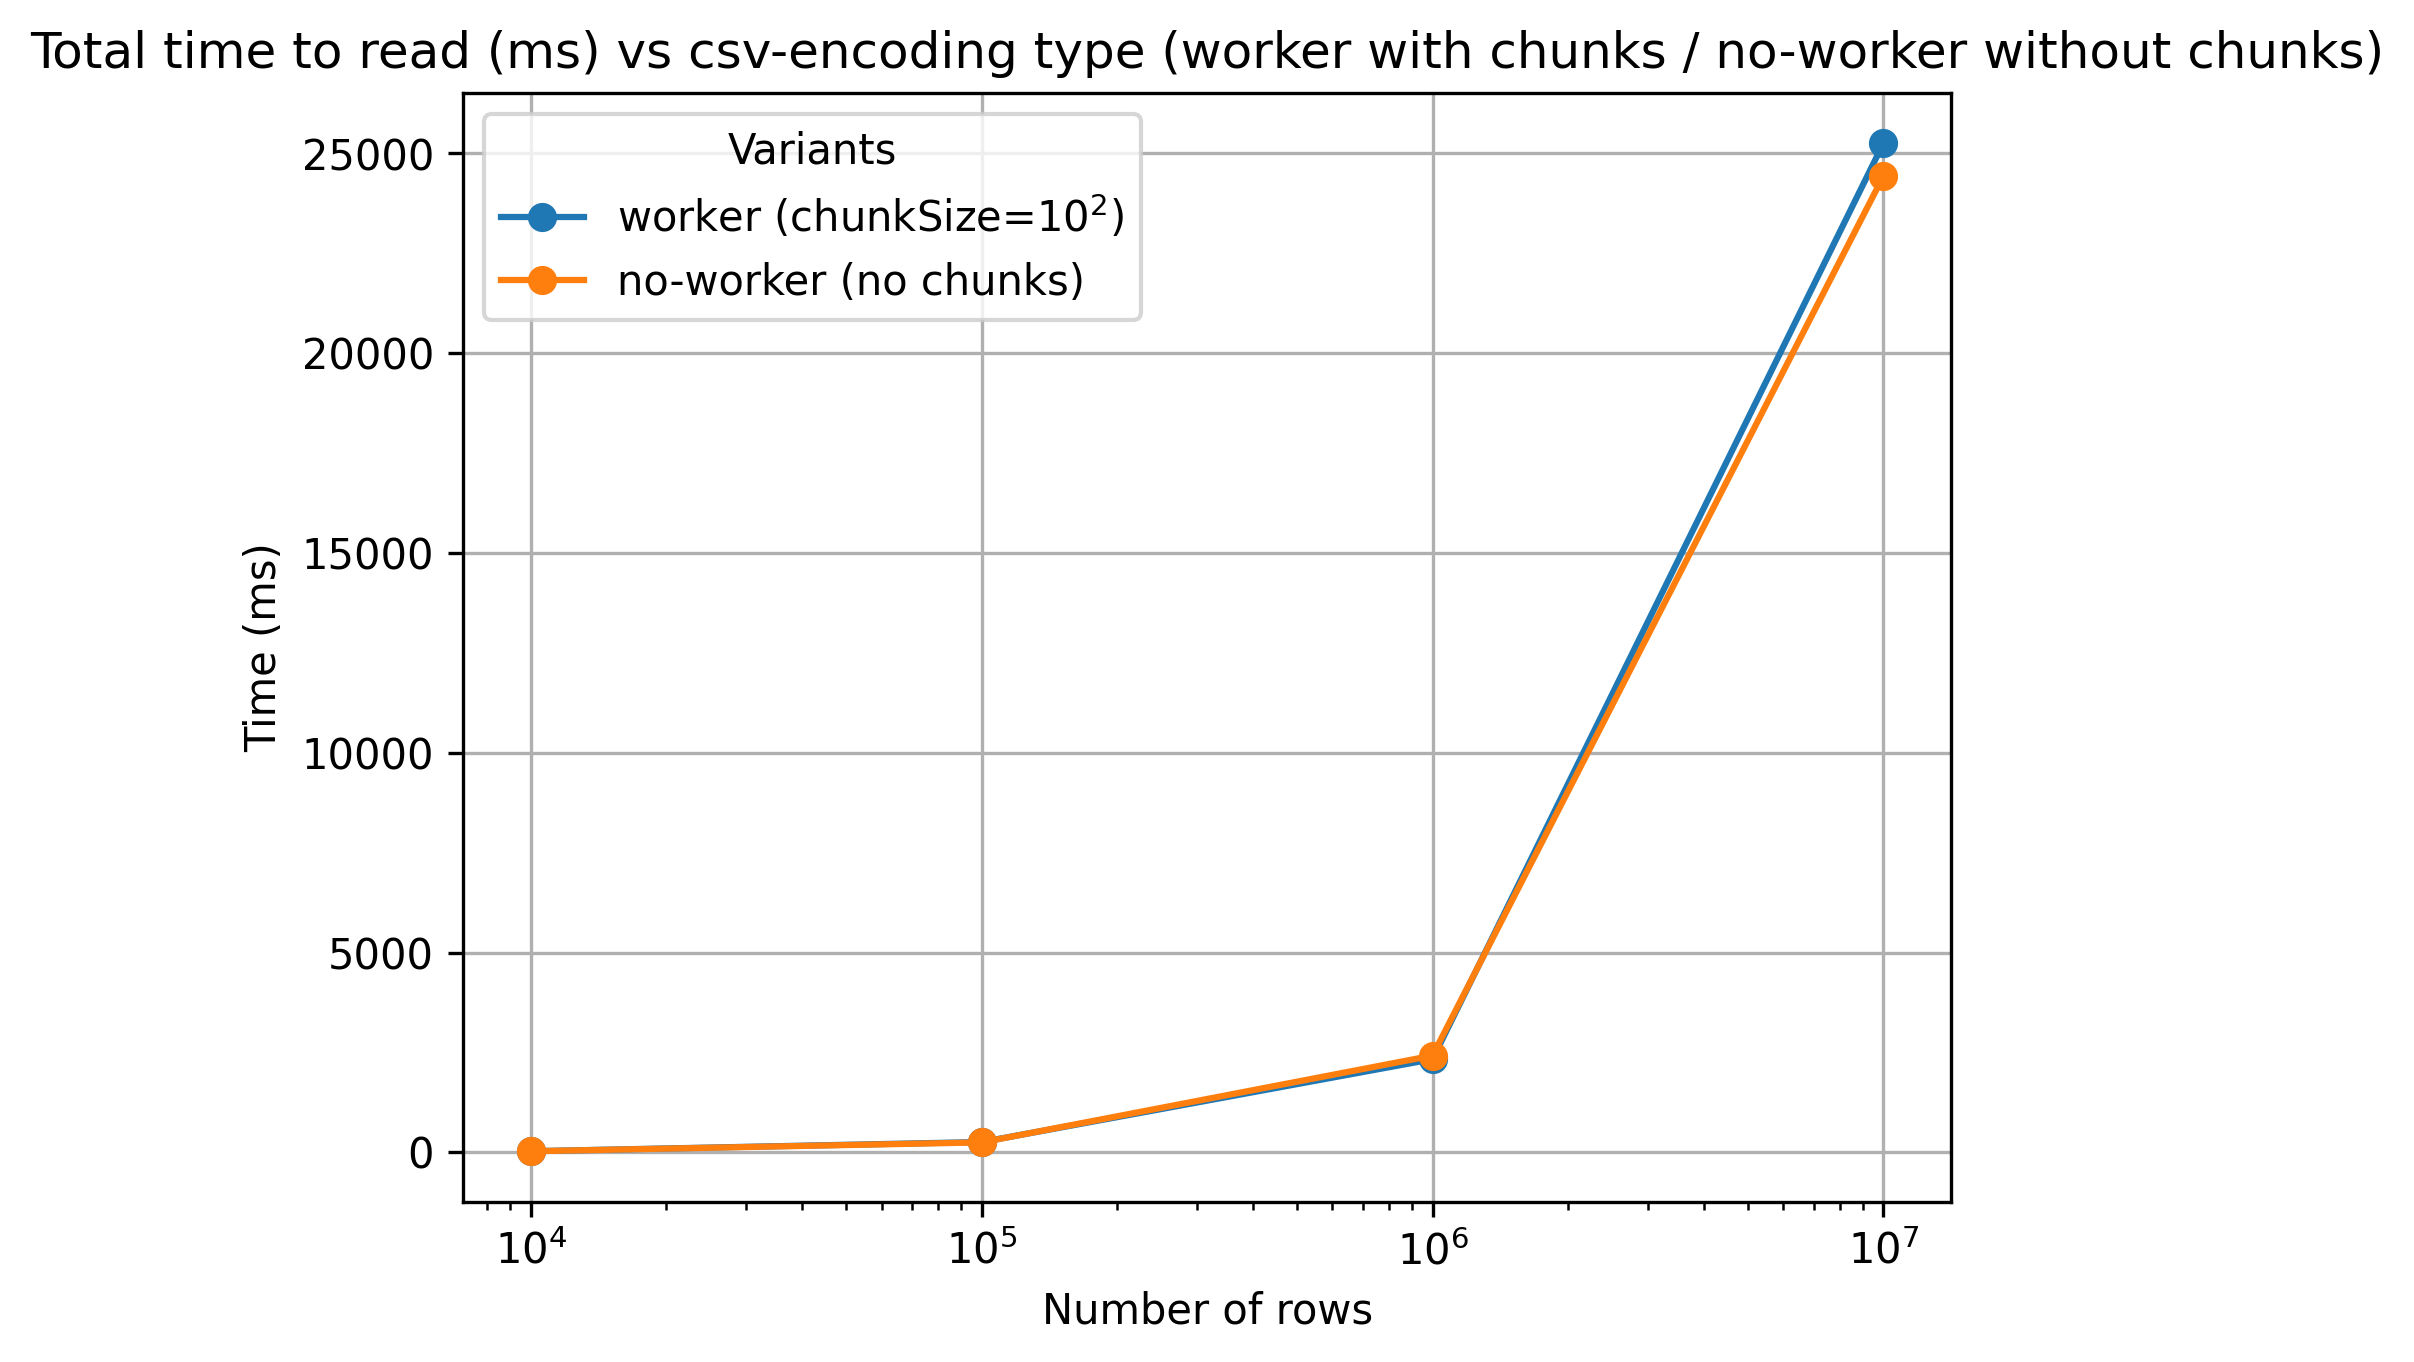
\includegraphics[scale = 0.7]{images/4-Experiments/read-input-csv-encoding-all.png}
  \caption{Comparison of \texttt{csv/encoding} variants up to $10^7$ rows}
\end{figure}

\begin{figure}[H]
  \centering
  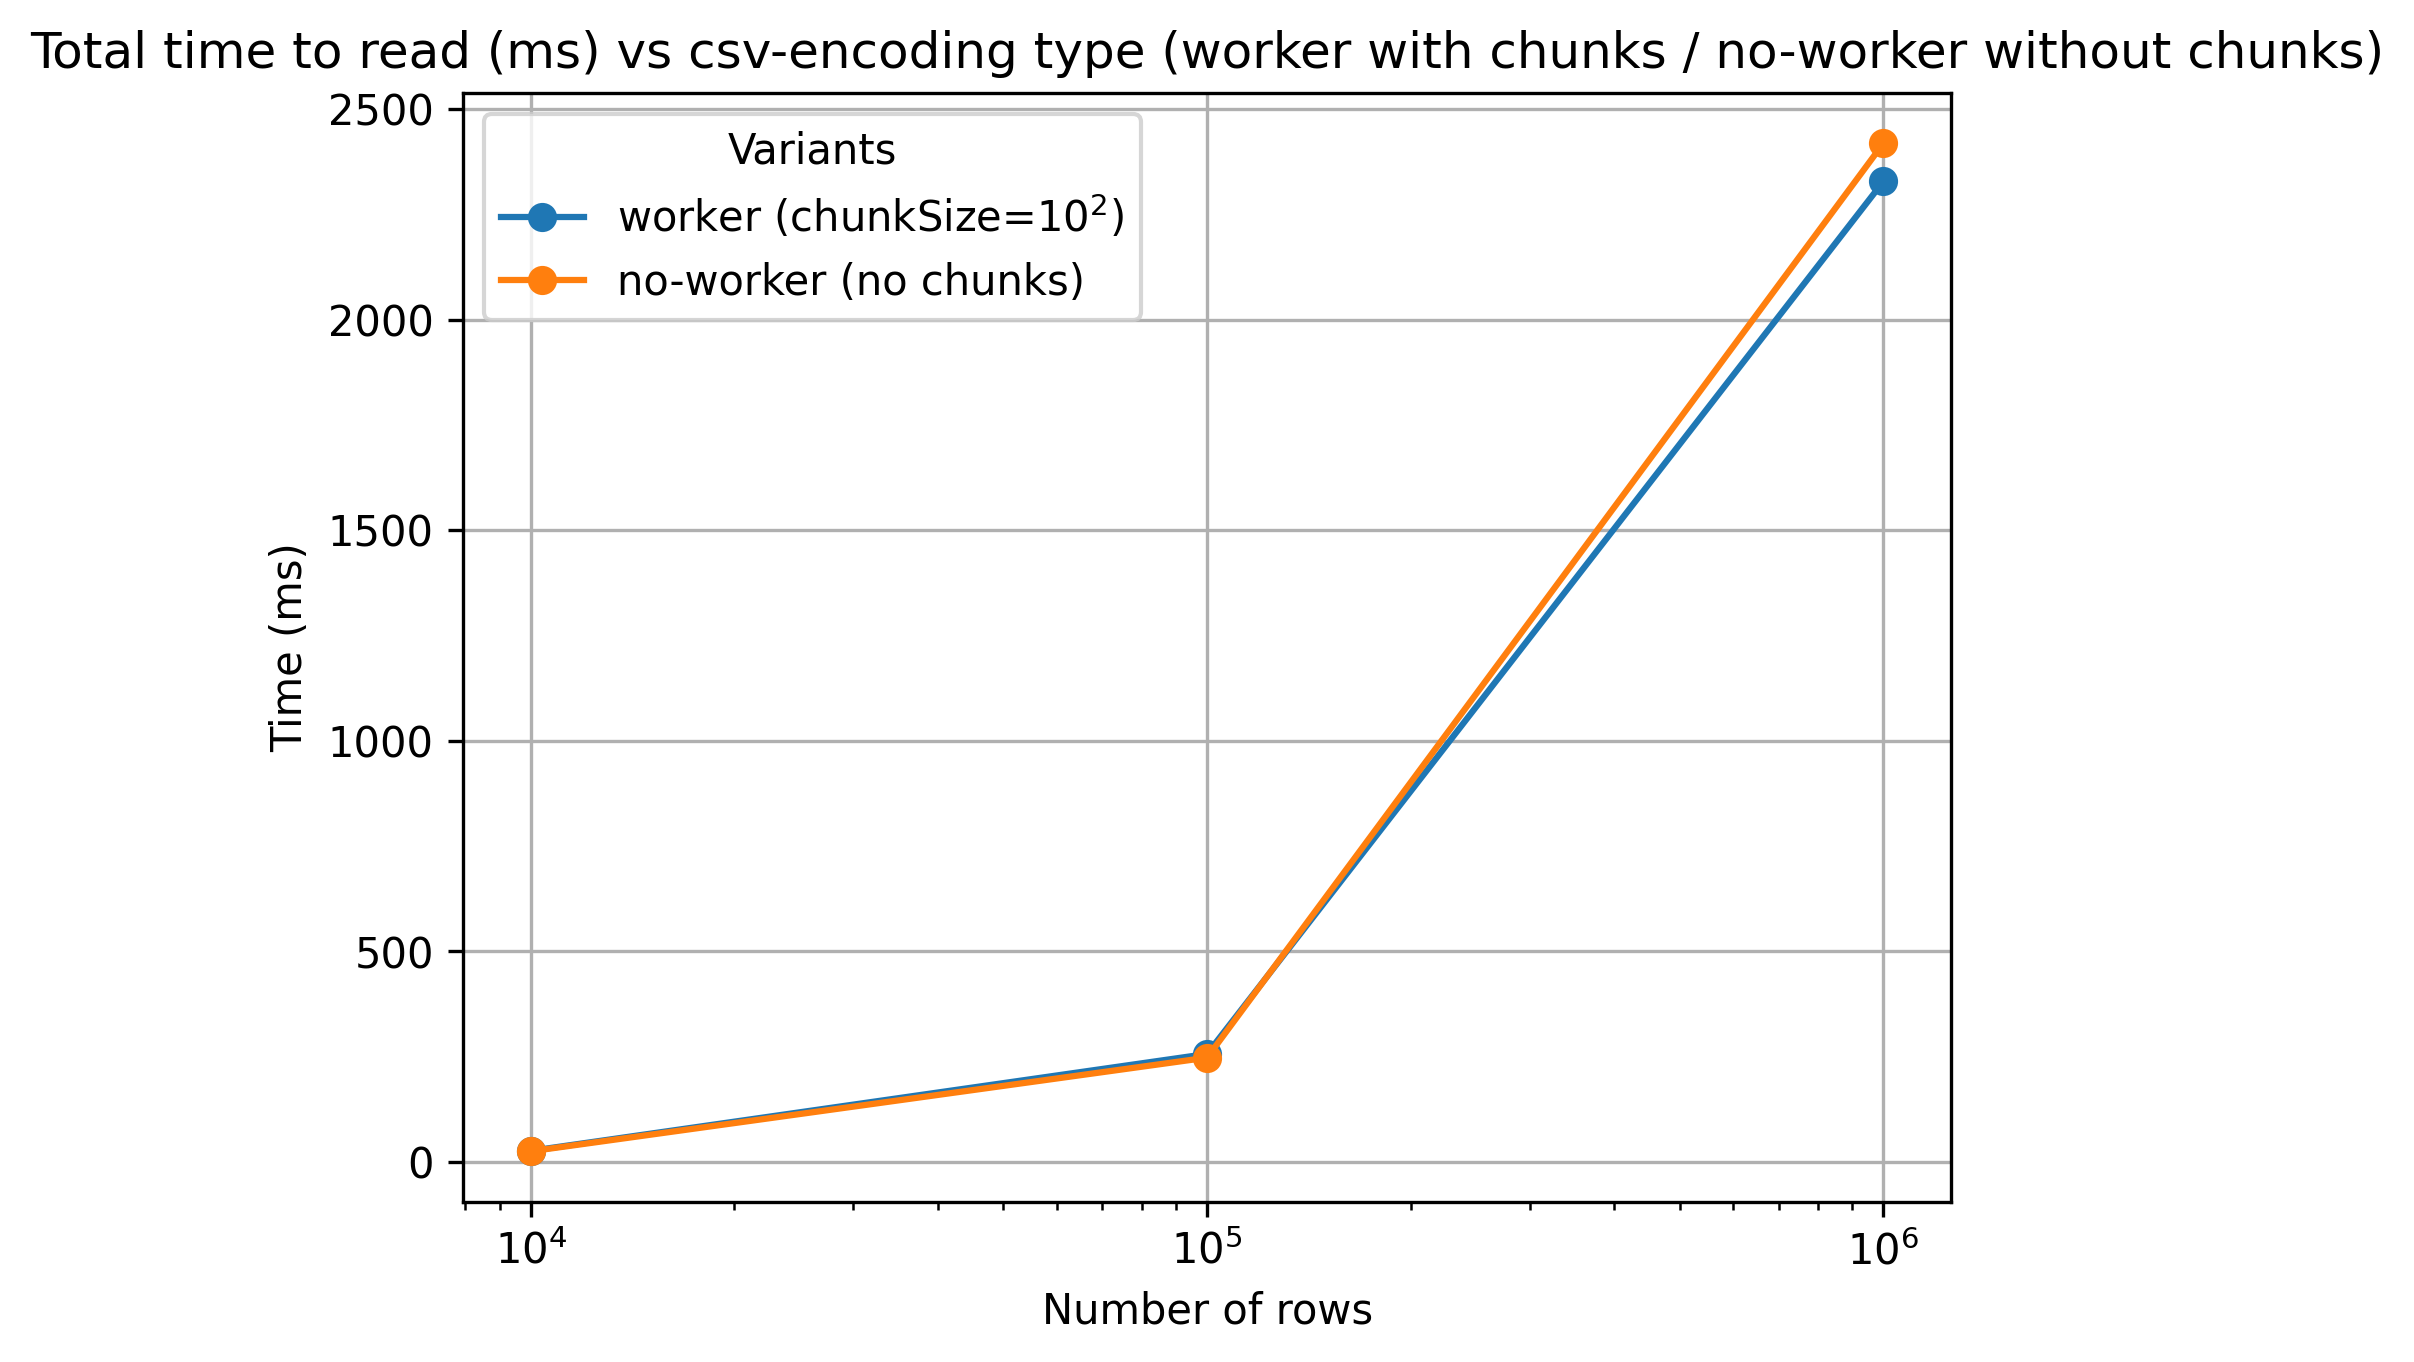
\includegraphics[scale = 0.7]{images/4-Experiments/read-input-csv-encoding.png}
  \caption{Comparison of \texttt{csv/encoding} variants up to $10^6$ rows}
\end{figure}

\begin{itemize}
  \item Differences insignificant
  \item Depend on the application
  \item Real-time simulation: worker version. To avoid possible bottleneck on the input reading. Instead the bottleneck be just the stopping to provide the input.
\end{itemize}

\textcolor{blue}{As it can be seen, the differences are insignificant, and the selection of each of the variants will depend on the application. For example, we suspect that the worker version can be beneficial in the real time simulation, so that we do not make the reading be the bottleneck of the simulation, by having a background process reading input transactions from the stream files while the main process providing the input to the pipeline can be stopped doing the real time simulation.}

\textcolor{red}{TODO: Comparativa run same experiment NRT with worker VS without worker for the input providing - a single experiment example to show that is better with worker!}

Some (other) references:

\begin{itemize}
  \item \href{https://www.confluent.io/es-es/learn/apache-flink/}{Apache Flink}: distributed processing engine for stateful computation of data streams.
\end{itemize}

\end{document}
